%% 
%% Copyright 2007-2020 Elsevier Ltd
%% 
%% This file is part of the 'Elsarticle Bundle'.
%% ---------------------------------------------
%% 
%% It may be distributed under the conditions of the LaTeX Project Public
%% License, either version 1.2 of this license or (at your option) any
%% later version.  The latest version of this license is in
%%    http://www.latex-project.org/lppl.txt
%% and version 1.2 or later is part of all distributions of LaTeX
%% version 1999/12/01 or later.
%% 
%% The list of all files belonging to the 'Elsarticle Bundle' is
%% given in the file `manifest.txt'.
%% 
%% Template article for Elsevier's document class `elsarticle'
%% with harvard style bibliographic references

\documentclass[final,times,twocolumn,article]{elsarticle}

%% For including figures, graphicx.sty has been loaded in
%% elsarticle.cls. If you prefer to use the old commands
%% please give \usepackage{epsfig}

%% The amssymb package provides various useful mathematical symbols
\usepackage{amssymb}
\usepackage{lipsum}
\usepackage{subcaption}
\usepackage{placeins}
\usepackage{fancyhdr}
\usepackage{amsmath}
\usepackage{hyperref}
\graphicspath{{/Users/carlafeliu/Docs/Master/TFM/github/TFM/output/}} %%Path from the figures


%% The lineno packages adds line numbers. Start line numbering with
%% \begin{linenumbers}, end it with \end{linenumbers}. Or switch it on
%% for the whole article with \linenumbers.
%% \usepackage{lineno}

%% You might want to define your own abbreviated commands for common used terms, e.g.:
%%\newcommand{\kms}{km\,s$^{-1}$}
%%\newcommand{\msun}{$M_\odot}

%%\journal{Astronomy $\&$ Computing}

\pagestyle{fancy}
\fancyhead{}
\fancyhead[RO]{\small Discovering cysteine protease covalent inhibitors using deep learning}
\fancyhead[LO]{\small Omics Data Analysis 2023}
%%\fancyfoot{}
%%\fancyfoot[LO]{\small September 2023}


\begin{document}

\begin{frontmatter}

%% Title, authors and addresses

%% use the tnoteref command within \title for footnotes;
%% use the tnotetext command for theassociated footnote;
%% use the fnref command within \author or \affiliation for footnotes;
%% use the fntext command for theassociated footnote;
%% use the corref command within \author for corresponding author footnotes;
%% use the cortext command for theassociated footnote;
%% use the ead command for the email address,
%% and the form \ead[url] for the home page:
%% \title{Title\tnoteref{label1}}
%% \tnotetext[label1]{}
%% \author{Name\corref{cor1}\fnref{label2}}
%% \ead{email address}
%% \ead[url]{home page}
%% \fntext[label2]{}
%% \cortext[cor1]{}
%% \affiliation{organization={},
%%            addressline={}, 
%%            city={},
%%            postcode={}, 
%%            state={},
%%            country={}}
%% \fntext[label3]{}

\title{Discovering cysteine protease covalent inhibitors using deep learning}

%% use optional labels to link authors explicitly to addresses:
%% \author[label1,label2]{}
%% \affiliation[label1]{organization={},
%%             addressline={},
%%             city={},
%%             postcode={},
%%             state={},
%%             country={}}
%%
%% \affiliation[label2]{organization={},
%%             addressline={},
%%             city={},
%%             postcode={},
%%             state={},
%%             country={}}

\author{Author: Carla Feliu Farré}
\author{Tutor: Jordi Villa Freixa}
\date{September 2023}
\affiliation{organization={Universitat de Vic - Universitat Central de Catalunya (UVic-UCC)}
            }
\affiliation{organization = {Department of Biociences, UVic-UCC}}

\begin{abstract}
%% Text of abstract
Cysteine proteases, are vital enzymes to biological processes but can contribute to diseases when dysregulated. Covalent inhibitors, which form stable bonds with target molecules, offer potential benefits. This study, explores the use of Artificial Neural Networks (ANNs) to identify covalent targets for cysteine protease inhibition. The research aims to develop an efficient approach to drug discovery using deep learning techniques. 
The study involves selecting appropriate compound databases, one with known interactions with the target and two others without such interactions, for the purpose of making predictions. ANNs are trained using the prepared datasets containing known interaction activities, employing various training methodologies to explore and enhance the stability and predictive accuracy of the model when applied to the other datasets for generating predictions. These results are meticulously analyzed to assess the reliability of the predictions in the context of inhibitor discovery. 
This research highlights the potential of machine learning, particularly ANNs, as a powerful tool in streamlining the drug discovery process by facilitating the identification of promising compounds for covalent inhibition.


\end{abstract}

%%Graphical abstract
%\begin{graphicalabstract}
%\includegraphics{grabs}
%\end{graphicalabstract}

%%Research highlights
%\begin{highlights}
%\item Research highlight 1
%\item Research highlight 2
%\end{highlights}

\begin{keyword}
%% keywords here, in the form: keyword \sep keyword, up to a maximum of 6 keywords
Cysteine protease \sep Deep learning \sep Artificial Neural Networks \sep Covalent inhibitors \sep MPNN

%% PACS codes here, in the form: \PACS code \sep code

%% MSC codes here, in the form: \MSC code \sep code
%% or \MSC[2008] code \sep code (2000 is the default)

\end{keyword}


\end{frontmatter}



%% main text

\section{Introduction}

Proteases, also known as peptid hydrolases, are enzymes capable of catalysing hydrolytic reactions that degrade protein molecules to peptides, and finally to free amino acids. They regulate various enzymatic cascades that form part of metabolic cycles \cite{Ramos2019}. The role they play is key in carrying out vital biological processes, such as the regulation of various cellular processes as well as differentiation, gene expression and cell death. Proteases constitute an extensive group of enzymes, classified based on various factors, including the specific amino acid residue present at their catalytic site. Commonly recognized subgroups include serine proteases, cysteine proteases, aspartic proteases, and metalloproteases, among others. This diversity is crucial for proteases to fulfill fundamental roles in numerous biological processes \cite{Ramos2019}.

Cysteine proteases (also known as thiol proteases), are characterised by catalysing the breakdown of proteins by cleavage of peptide bonds using a cysteine nucleophile thiol. These proteases are classified into two types according to their location within the organism; Cathepsins, located in the lysosome, and Calpains, located in the cytosol \cite{Gupta2020}. Having a catalytic dyad or triad, which includes a cysteine (active site), proximately of an histidine. Depending on the type of cysteine proteases, can be Cys-His (Cysteine - Histidine) or Cys-His-Asp (Cysteine - Histidine - Aspartic acid)\cite{Nicholson2013}. (Figura XXXX) 

Although these proteases have a key role in vital processes, when there is overexposure or dysregulation in pathological conditions, they can contribute to the development of many diseases. Search for inhibitors of cystein proteases has become an objective in medical and pharmacological research, in order to develop new therapeutic opportunities \cite{cath}. In several studies, it has been shown that cathepsins, are related to tumour progression \cite{Berdowska2004} \cite{Mohamed2006}. These cysteine proteases allow cancer cells to attack nearby tissues, blood and lymphatic vessels and metastasise to peripheral tissues \cite{Gupta2020} \cite{Gocheva2006}.

 They represents interesting pharmacological targets due to the reactivity of the cysteine in the active site. The high nucleophilicity of the cysteine thiol under physiological conditions provides an ideal anchoring site for small electrophilic molecules. \cite{Maurais2019} 

The inhibition process is defined by the effectiveness of the binding of a protein to the selected targets. This depends on the molecular reactions between the functional groups of the drug and the active site residues of the protein. The final interactions can be either covalent or non-covalent. 
Covalent bonds are usually formed by the interaction of certain amino acids, including the nucleophilic cysteine and a reactive functional group of the ligand. They are more effective than non covalent inhibitors due to their long permanence in the active site and high binding affinity resulting in complete inhibition of the target compared to the reversible effect of non-covalent drugs. \cite{Aljoundi2020} 


The drug development process is a very elaborate process, which can involve a lot of time and resources. It begins with the search for and characterisation of a possible biological target for a specific disease or enzyme, and then the process of creating the most suitable therapeutic compound begins. Before reaching drug development, many molecular properties must be optimised to identify and validate the target, as this is one of the most important steps in drug development. \cite{Hughes2011}
Historically, this search was guided by the calculations and intuition of expert scientists, but with the great advances in new technologies and the increase in resources, it has been possible to apply new methods that are much faster and more reliable. \cite{Hop2018}


Machine Learning (ML), particularly Deep Learning (DL), has proven highly effective in diverse chemistry applications. Unlike traditional physical models relying on specific equations, ML uses various algorithms to establish patterns for predicting novel compound properties in chemistry, biology, and physics. This approach has thrived with the increasing quantity and quality of available data, making it an optimal choice for solving problems with abundant data and variables but no known model or formula to relate these variables among themselves with the expected outcome. In drug discovery, the shift toward to large datasets led to the evolution of ML into DL. These is built upon artificial neural networks (ANN), allowing computer systems to make predictions or decisions based on past experiences without explicit programming \cite{Nag2022}.

Artificial neural networks, are created to simulate a network of model neurons on a computer. Applying algorithms that mimic the processes of real neurons, models are generated that learn to solve many types of problems. The networks are composed of artificial neuron units, capable of transmitting signals to each other. Each reception of a signal in the neurons is associated with a weight that varies as learning progresses, which can increase or decrease the strength of the signal that will then be sent to the other neurons. These signals pass the multilayers of artificial neurons until they reach the final layer, where the result of these connections is the prediction of the algorithm. \cite{Talevi2020} \cite{Nag2022}

\begin{figure}[h]
    \centering 
     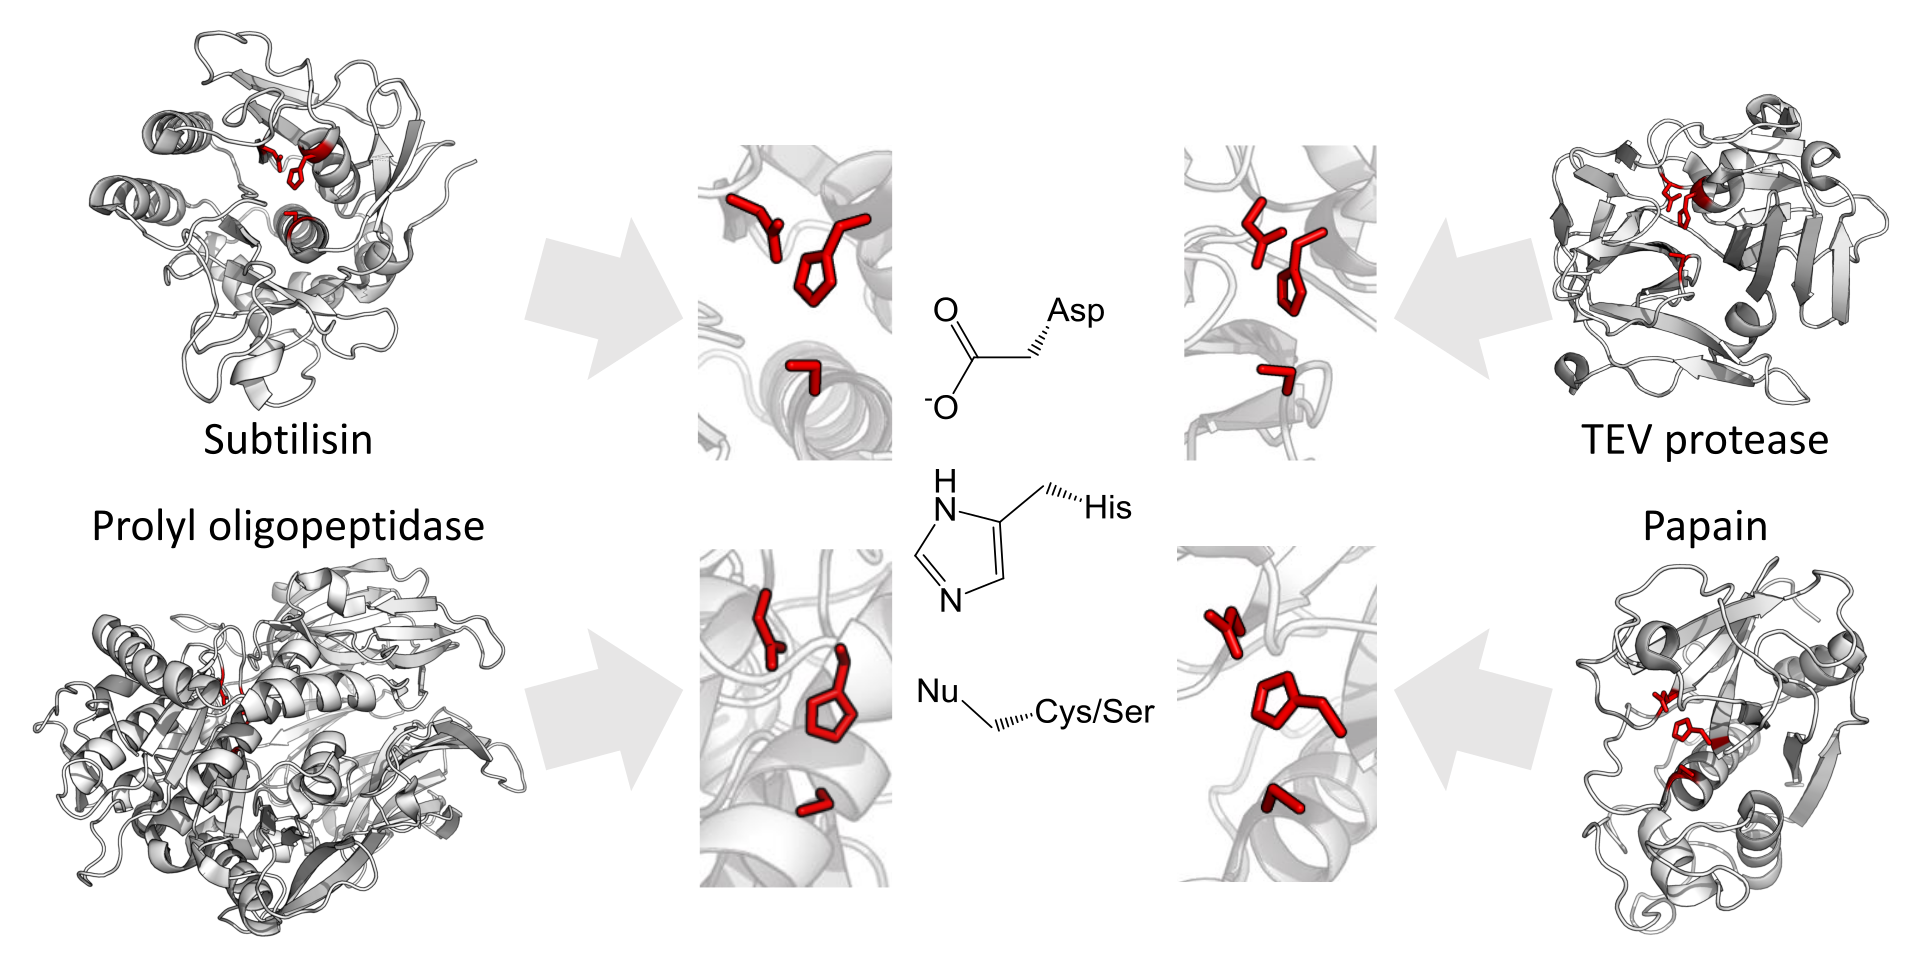
\includegraphics[width=0.4\textwidth]{Triad_convergence_ser_cys.png}	
     \caption{In the figure, con be observed the organization of catalytic involving systeine and serine residues. It illustrates how these triads interact with the active site of enzimes such as subtilisin, prolyl oligopeptidase, TEV protease and papain. These triads have converged to nearly identical arrangements, driven by the mechanistic similarities between cysteine and serine proteolysis mechanisms.} 
     \label{Figure1}
 \end{figure}

\begin{figure}[h]
    \centering 
     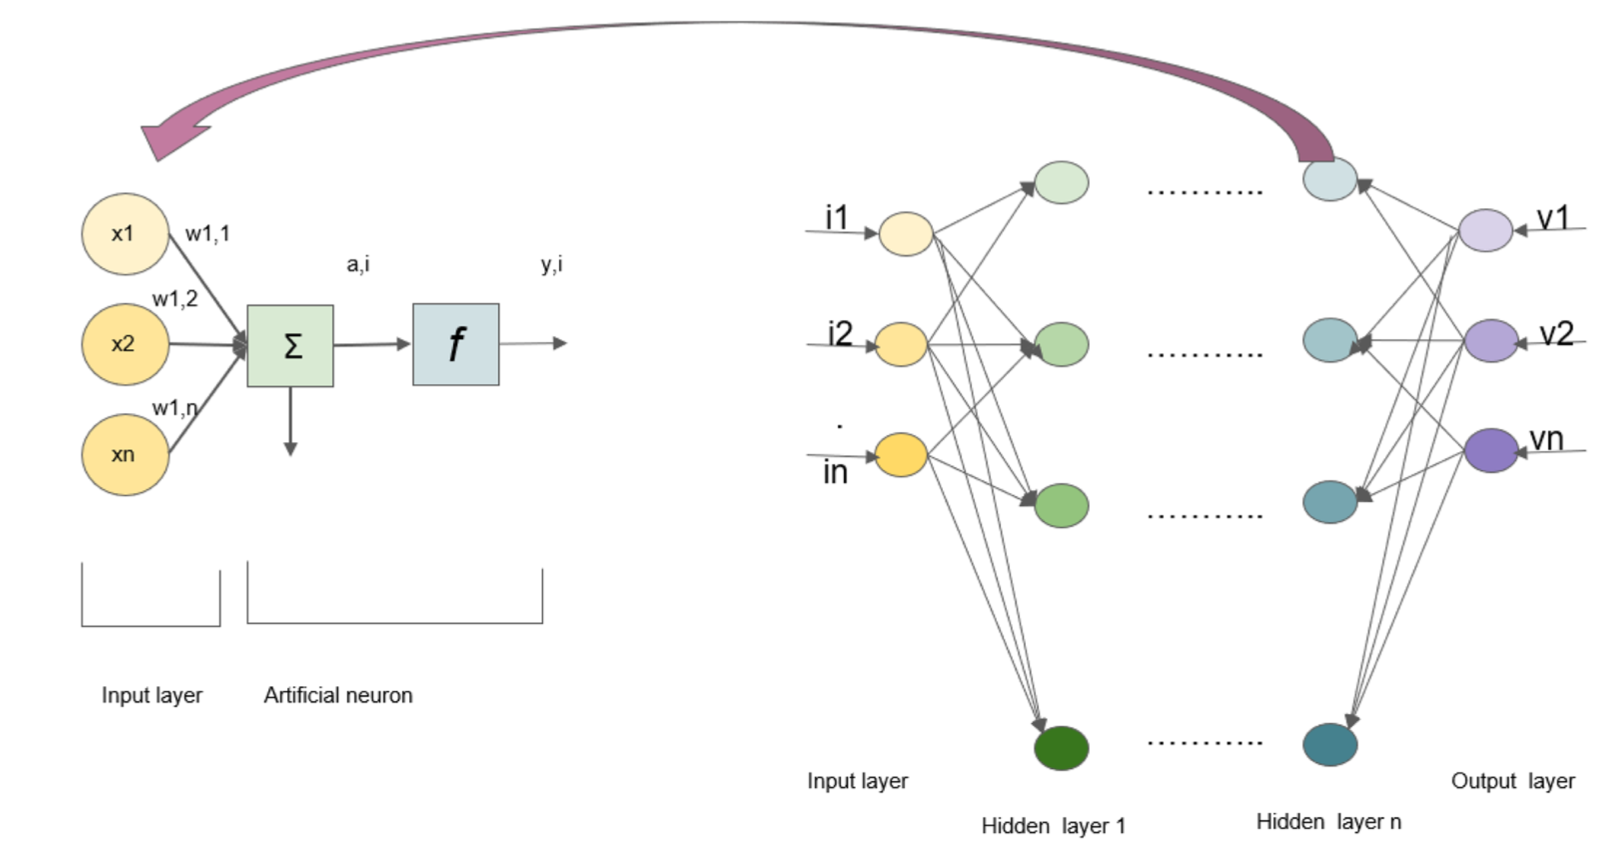
\includegraphics[width=0.4\textwidth]{Schematic_diagram_ANN_(Introduction).png}	
     \caption{Schematic diagram that illustrates how a single neuron functions within an artificial neural network (ANN). The performance of the ANN depends on factors such as the number of layers it has, the number of neurons, how they communicate with each other, the bias, and the mathematical operations they perform to transform information. The figure shows various input data (i1,i2..) and output data (v1,v2...) which are depicted as small neurons connected to each other.} 
     \label{Figure2}
 \end{figure}

The chemprop Architecture is a neural network built for the prediction of molecular properties that includes a directed message passing neural network (D-MPNN) module for molecular feature extraction and a feed-forward neural network (FNN) for property prediction. The Directed Message Passing Neural Network (D-MPNN) model is a variation of the Message Passing Neural Network (MPNN) architecture built upon an existing Graph Convolutional Network (GCN). The primary distinction between D-MPNN and conventional MPNN lies in the nature of the messages transmitted throughout the molecule during message passing \cite{Yang2019}. A feed-forward neural network, operates without loops in its node connections, ensuring that information flows strictly in a forward direction without any feedback loops \cite{Wallisch2009}.
This model takes molecular SMILES as input and extracts all the atomic and bonding characteristics of the molecules to generate a single vector of characteristics which, by entering it into the FNN, can predict the activity of the candidate molecules. \cite{Wang2022}

Given the growing interest in cysteine proteases as targets for therapeutic treatments and the availabikity of new machine learning tools for these drug discovery processes, one question is raised in this work.

\begin{itemize}
    \item Can ANN be used to identify potential covalent targets and molecular patterns for cysteine protease inhibitors in diverse databases?
    %%\item What is the best way to train a model using ANN?

    
\end{itemize}

Specific objectives:

\begin{enumerate}
    \item Identify a database with known targets of cysteine proteases that includes inhibitory activity, which will serve as the training data of our ML model. 
    \item Download the database and extract the (Simplified Molecular Input Line Entry Sistem)SMILES information. Prepare the required dataframe structure for working with the ML algorithm, obtaining various features for each molecule and its inhibitory activity (IC50).
    \item Train the chemprop model using various approaches, evaluating which one makes the model more stable for our predictions. 
    \item Identify suitable databases to obtain the molecules for our predictions. Similar to the training dataframe, construct the structure necessary to make the predictions with our training model. 
    \item Analyze the data generated from the predictions made by the ML model, checking the correlation of the data and their similarity to understand if the predictions obtained are suitable for our questions raised. 
    \item Detect patterns of molecules that could be optimal for working in the discovery of cystein protease inhibitors. 
\end{enumerate}

\section{Methods}

\subsection{Datasets}

In this study, we worked with three different databases to extract the necessary information for our research. Data extraction has been performed depending on each database.  

\subsubsection{ChEMBL}

ChEMBL is a database of bioactive small molecules similar to drugs, containing calculated properties and bioactivities. \cite{chemblweb}

Our interest in this database is to obtain information about molecules that can interact with cysteine proteases in order to establish a reference point for interaction activity, allowing us to train our ML model. To access the relevant information to our study, we filtered the ChEMBL database with the term "cysteine protease" and extract the resulting targets. Once we obtained the cysteine protease targets, we used the python "requests" module to retrieve information about all the molecules interacting with each of the targets, along with their interaction activity, represented by the -log(IC50 molar) value. The value was used to train our ML model. 

\subsubsection{ChemDiv}

ChemDiv is a globally recognized research organization in drug discovery solutions. They have identified specific libraries aimed at addressing varius targets, protein domains, cellular processes and more. \cite{chemdivweb}

From this database, we obtained the "Cysteine Targeted Covalent Library", which consists of 39,301 compounts with specific warheads designed to react with cysteine. The objective of using this library is, by applying our trained model, to find possible compounds that exhibit significant interaction activity with cysteine. This will help us identify patterns that can be used to understand what type of molecule could be a good inhibitor. 

\subsubsection{Zinc}

ZINC is a database that houses an extensive collection of commercially available chemical compounds used in virtual screening and drug design research. \cite{zincweb}

Given that this database contains a vast amount of information, with over 230 million compounds, we have randomly selected a portion of this data to conduct our analysis. From the database, we extracted a .uri document containing .url links to different segments of information within the zinc database. Using a Python function, we collected information from three of these files to conduct an analysis of a portion of the zinc data. This has allowed us to work with a more manageable amount of data and focus our objective on applying the algorithm to a comprehensive database.


\subsection{Machine learning model}

To carry out the study and work with the Machine Learning algorithm, we have used the the Visual Studio Code editor to generate all the necessary code in the python programming lenguage. 

Machine Learning is an expansive field where various algorithms and models can be used to achieve multiple objectives. In this study, we developed code that uses a deep learning model incorporating a directed message passing neural network (D-MPNN) to obtain predictions. 

We employed the Chemprop architecture, an open-source machine learning framework. This framework includes a D-MPNN module for molecular feature extraction and a feed-forward neural network (FNN) for property prediction. To work with this algorithm, input in SMILES format (representing chemical formulas) is required. The algorithm then transforms this input into a molecular graph structure, where atoms serve as nodes, and bonds as edges. 

The D-MPNN module is a critical component responsible for extracting distinctive characteristics from individual atoms, effectively constructing a comprehensive dataset that represents the entire molecule. This process involves a one-way flow of information, starting from the input layer and culminating in the final output layer. The resulting vector, which encapsulates the molecule's essential features, is subsequently utilized in the FNN module to make predictions concerning the activity of the studied molecules. This sequential data flow ensures that relevant information is systematically incorporated into the predictive modeling process, enhancing its accuracy and effectiveness. \cite{Wang2022}

A deep learning artificial neural network can solve classification or regression problems. Classification problems involve the use of labels, where data must be categorized into multiple categories. On the other hand, regression problems require the specification of a numerical quantity to classify variables. In this work, we have focused on regression problems, using the IC50 value variable extracted from the ChEMBL database, which classifies molecules on their interaction activity. 

\subsection{pIC50}

The inhibition constant IC50 value is a quantitative measure of a substance's potency in inhibiting a specific biological or chemical function. It signifies the amount of a particular inhibitory substance required to inhibit a specific biological component in 50\%. pIC50 is a logarithmic transformation of IC50 values: 
\begin{equation}
    pIC_{50} = -\log_{10}(IC_{50})
\end{equation}
Higher values of pIC50 indicate exponentially more potent inhibitors \cite{pic50}.

\subsection{Data preparation and curation}

To carry out the process of training machine learning models effectively, it is crucial to have suitable and properly prepared dataset. Therefore, prior preparation is required. 

This data structure should have a first column containing the SMILES of the molecules, features describing the molecules, and finally, in a last row, the interaction activity of these molecules, the IC50 value. Data preparation also includes conducting a thorough analysis of the data structure, which is essential for a deep understanding of the data and, consequently, for conducting a more accurate result analysis. 

\subsubsection{ANN training}

To prepare the training data, we started with a list of all the targets that interact with cysteine proteases and their interactions, from the ChEMBL database. These initial data will provide us a lot of information, but there is an important data preprocessing step before introducing the dataframe into our model. 

From this dataframe containing the ligands of the cysteine protease targets, we extracted the list of all the ChEMBL IDs of the molecules that interact with them, along with their IC50 activity values. Using a ChEMBL API and Python function, we obtained the SMILES for each of the registered molecules. 

The data cleaning process is very important, which includes the removal of null values, as they represent a lack of information that may not be accepted or could influence the outcome of the algorithm, and the elimination of duplicated SMILES to avoid duplicated information. 

To prepare the training data, we used the chemoinformatics and machine learning software RDKit \cite{rdkitweb}. From this software, we employed a Python function to iterate over each SMILE, resulting in a total of 10 different features extracted from each compound. Once we had the data prepared, we used a .sh scripts with the necessary commands to work with the chemprop algorithm to perform the data training. 
In order to ensure and assess the quality of the trained model, we conducted four trainings using four slightly different feature dataframes. These dataframes were analyzed, and ultimately, we determined which one is the most suitable for analyzind our data. 

\begin{itemize}
\item Train 1: No curated and no normalized data.
\item Train 2: Curated and no normalized data.
\item Train 3: Curated and z-score normalized data.
\item Train 4: Curated and MinMaxScaler normalized data.
\end{itemize}
\subsubsection{Ligand prediction}

The first prediction was carried out using data from ChemDiv. To extract this data, we specifically selected the ChemDiv Cysteine Targeted Covalent Library to obtain the initial results. 

We downloaded the ChemDiv library from the database using a Python script. The script provided an SDF file containing comprehensive information for each molecule. Utilizing a function that interfaces with RDKit module, we constructed a dataframe. This dataframe included the first column containing SMILES representations, followed by 10 different features for each molecule. Importantly, the pIC50 activity was omitted from the dataframe, as it will be acquired through the ML model.

To prepare the data for input into the algorithm, we performed a curation similar to the one mentioned in the training data preparation. Additionally, we added 200 molecules extracted from the dataframe used to train the model, as these molecules have been entered into the system with real and validated values, providing a reference. Finally, to ensure that the data have the same distribution to the trained model that will be used, we performed a normalization by rescaling all the data to a range of [0-1]. 

The second prediction was carried out with data from the general Zinc database. It was used to address the goal of finding patterns within a general database, without especificity to cysteine proteases. 

From Zinc, we retrieved a file with a .uri extension containing the complete database distributed across various URLs. Utilizing Python's wget module, we programmatically accessed these URLs and downloaded the data, yielding multiple files that collectively constitute the Zinc database. Following this, a Python script was employed to download three of these files. The resulting dataframe from this download comprises SMILES paired with their corresponding ZINC IDs. 

Through a function that uses RDKit, we filtered out invalid SMILES to minimize potential errors before preparing the dataframe for the algorithm. Similarly to what we mentioned earlier for the other dataframes, we used a function with RDKit to generate the appropriate matrix for inputting into the algorithm, with the first column containing the SMILES, followed by 10 features for each one. 

Finally, as we did with the first dataframe prediction, we added the same 200 molecules extracted from the training dataframe and normalized data by rescaling all the data to a range of [0-1].

\subsection{Results data analysis}

First and foremost, to analyse the training results, we will evaluate the metrics obtained from each of the training sessions:

\begin{itemize}
    \item Mean Absolute Error (MAE): MAE is a measure of the average difference between the model's predictions and the actual values. The closer MAE is to 0, the better the model's performance, as it indicates that the predictions are closer to the actual values.
    \item Mean Squared Error (MSE): MSE takes the square of the differences between predictions and actual values and calculates an average. The lower the value, the better the model's performance. 
    \item Coefficient of Determination ($R^2$): It is a measure that assesses how well the predictions fit the actual values. This value varies from 0 to 1, where 1 indicates a perfect fit to the model, and 0 indicates no fit at all. 
    \item Root Mean Squared Error (RMSE): RMSE is the square root of MSE and is used to provide an average of the model's error. The lower it is, the better the model's performance. 
    \end{itemize}

Once the result of the prediction from the used model was obtained, an analysis was conducted to assess the residual error of the resulting prediction. The 200 reference molecules, which were used both for training and obtaining the predictions, were used to generate a histogram and a regression line. This analysis allows us to visualize the model's error and the reliability of our data. 

To analyze and draw conclusions from the results, correlation graphs of the variables were generated for the two predictions made, in order to observe the relationship between all the calculated features. Additionally, a correlation graph of all the features with the pIC50 activity value calculated by the model was created. 

Finally, based on the results of the two predictions from the different databases, a selection of the molecules with a higher pIC50 value was made, generating a dataframe for each prediction of the 10 molecules showed stronger interactions. To conclude, a similarity analysis was conducted. To perform the similarity analysis, the Tanimoto coefficient, or Jaccard-Tanimoto index was used, which compares the similarity between two sets of samples. The results it provides are measured on a scale from 0 to 1, with a result closer to 1 indicating a higher degree of similarity among the molecules \cite{Bajusz2015}. This will enable us to observe and analyze if there is a pattern among the molecules with higher activity, providing an indication of whether our model aligns with the objective or not. 

\section{Results}
%%\label{Results}

The different dataframes prepared for training the model originated from a dataset extracted from ChEMBL containing 19,262 molecules. In the case of train 1, a less elaborate data curation was performed, resulting in a dataframe with 19,172 molecules. For train 2, an enhanced data curation was undertaken, beginning with the same database. This process involved the removal of duplicate SMILES, resulting in a reduced dataset containing 11,703 unique molecules. Train 3 and Train 4 were then derived from the dataset generated in Train 2, with data normalization applied using the z-score and the MinMaxScaler methods, respectively. (Table~\ref{Table1})

\begin{table}[ht]
\centering
\begin{tabular}{l c c c} 
     \hline
     Train & Initial & Curated & Norm.\\ 
     \hline
     Train 1 & 19,262 & 19,172 & No\\
     \hline
     Train 2 & 19,262 & 11,703 & No \\
     \hline
     Train 3 & 19,262 & 11,703 & Z-Score\\ 
     \hline
     Train 4 & 19,262 & 11,703 & MinMaxScale\\ 
     \hline
    \end{tabular}
\caption{Training sets}
\label{Table1}
\end{table}

In both Table~\ref{Figure3} and Figures~\ref{Figure4} and ~\ref{Figure5}, the evaluation metrics of the training models are presented, where we can see the different results: 

\begin{itemize}
\item Mean Absolute Error (MAE): As can be seen in the results of the mentioned figures, training model 4 shows the best performance in this aspect, while training model 1 performs the worst.
\item Mean Squared Error (MSE): It can be observed that training model 4 continues to have the best performance, while training model 1 performs the worst.
\item Coefficient of Determination ($R^2$): That the model that approaches 1 the closest and therefore fits better is training model 2, followed by training models 4 and 3, which have the same $R^2$ value with very little difference from 2. Finally, training model 1 is the furthest from a perfect fit.
\item Root Mean Squared Error (RMSE): Training model 1 stands out by a significant margin as having the best performance.
\end{itemize}

The results obtained from the 4 training runs conducted with the ML model algorithm show that the model with the highest possibility of error is training model 1, prepared with less elaborate data curation and with non-normalized data, while the one with the most reliable prediction is training model 4, with stricter data curation and a MinMaxScaler normalization. With the training results analysis, it is decided to use Train 4 to obtain the predictions for our study. 

\begin{figure}[ht]
    \centering 
     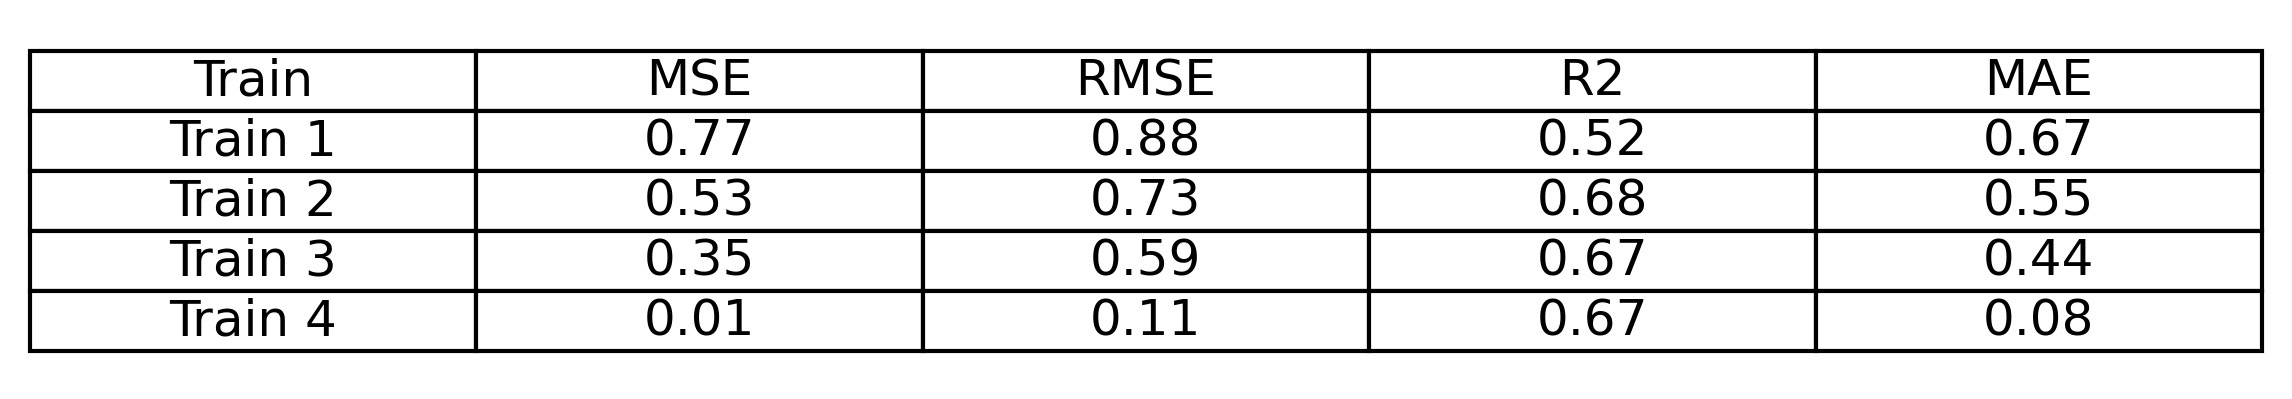
\includegraphics[width=0.4\textwidth]{results_train.jpeg}	
     \caption{Training set results metrics} 
     \label{Figure3}
 \end{figure}
 
 \begin{figure}[ht]
     \centering 
      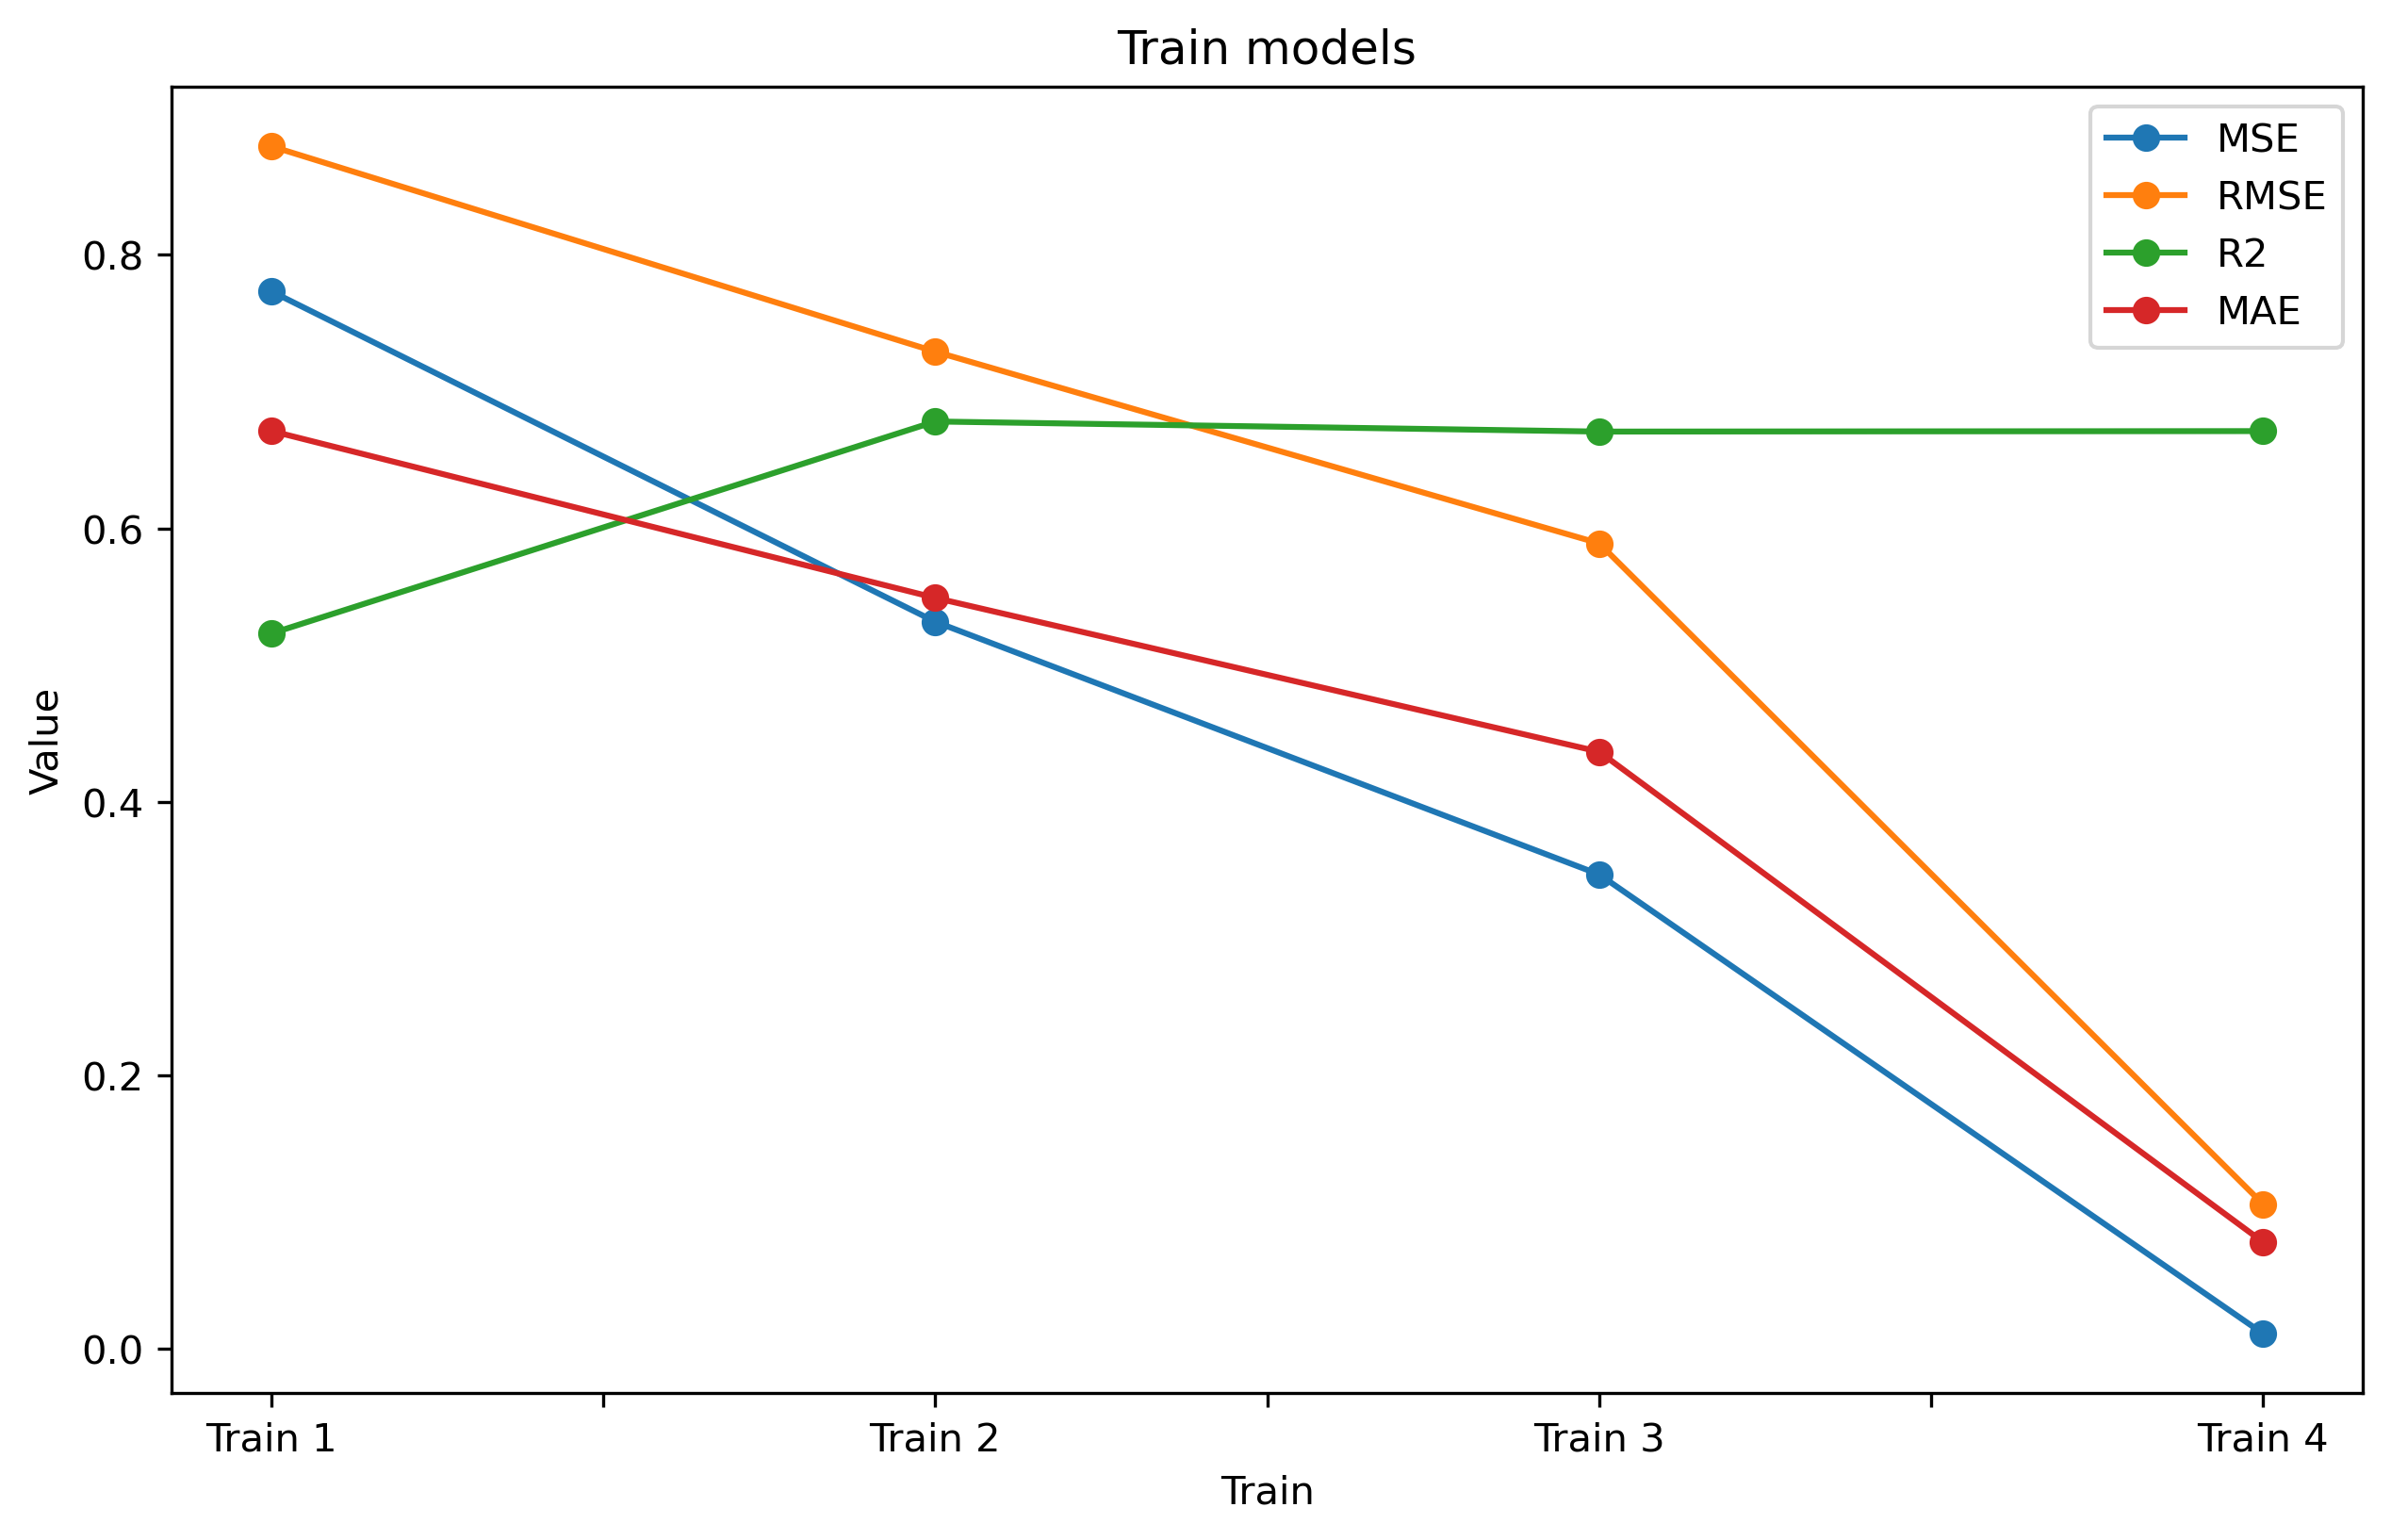
\includegraphics[width=0.4\textwidth]{plot_results_train.png}	
      \caption{Line chart of training set results metrics} 
      \label{Figure4}
  \end{figure}
 
  \begin{figure}[ht]
     \centering 
      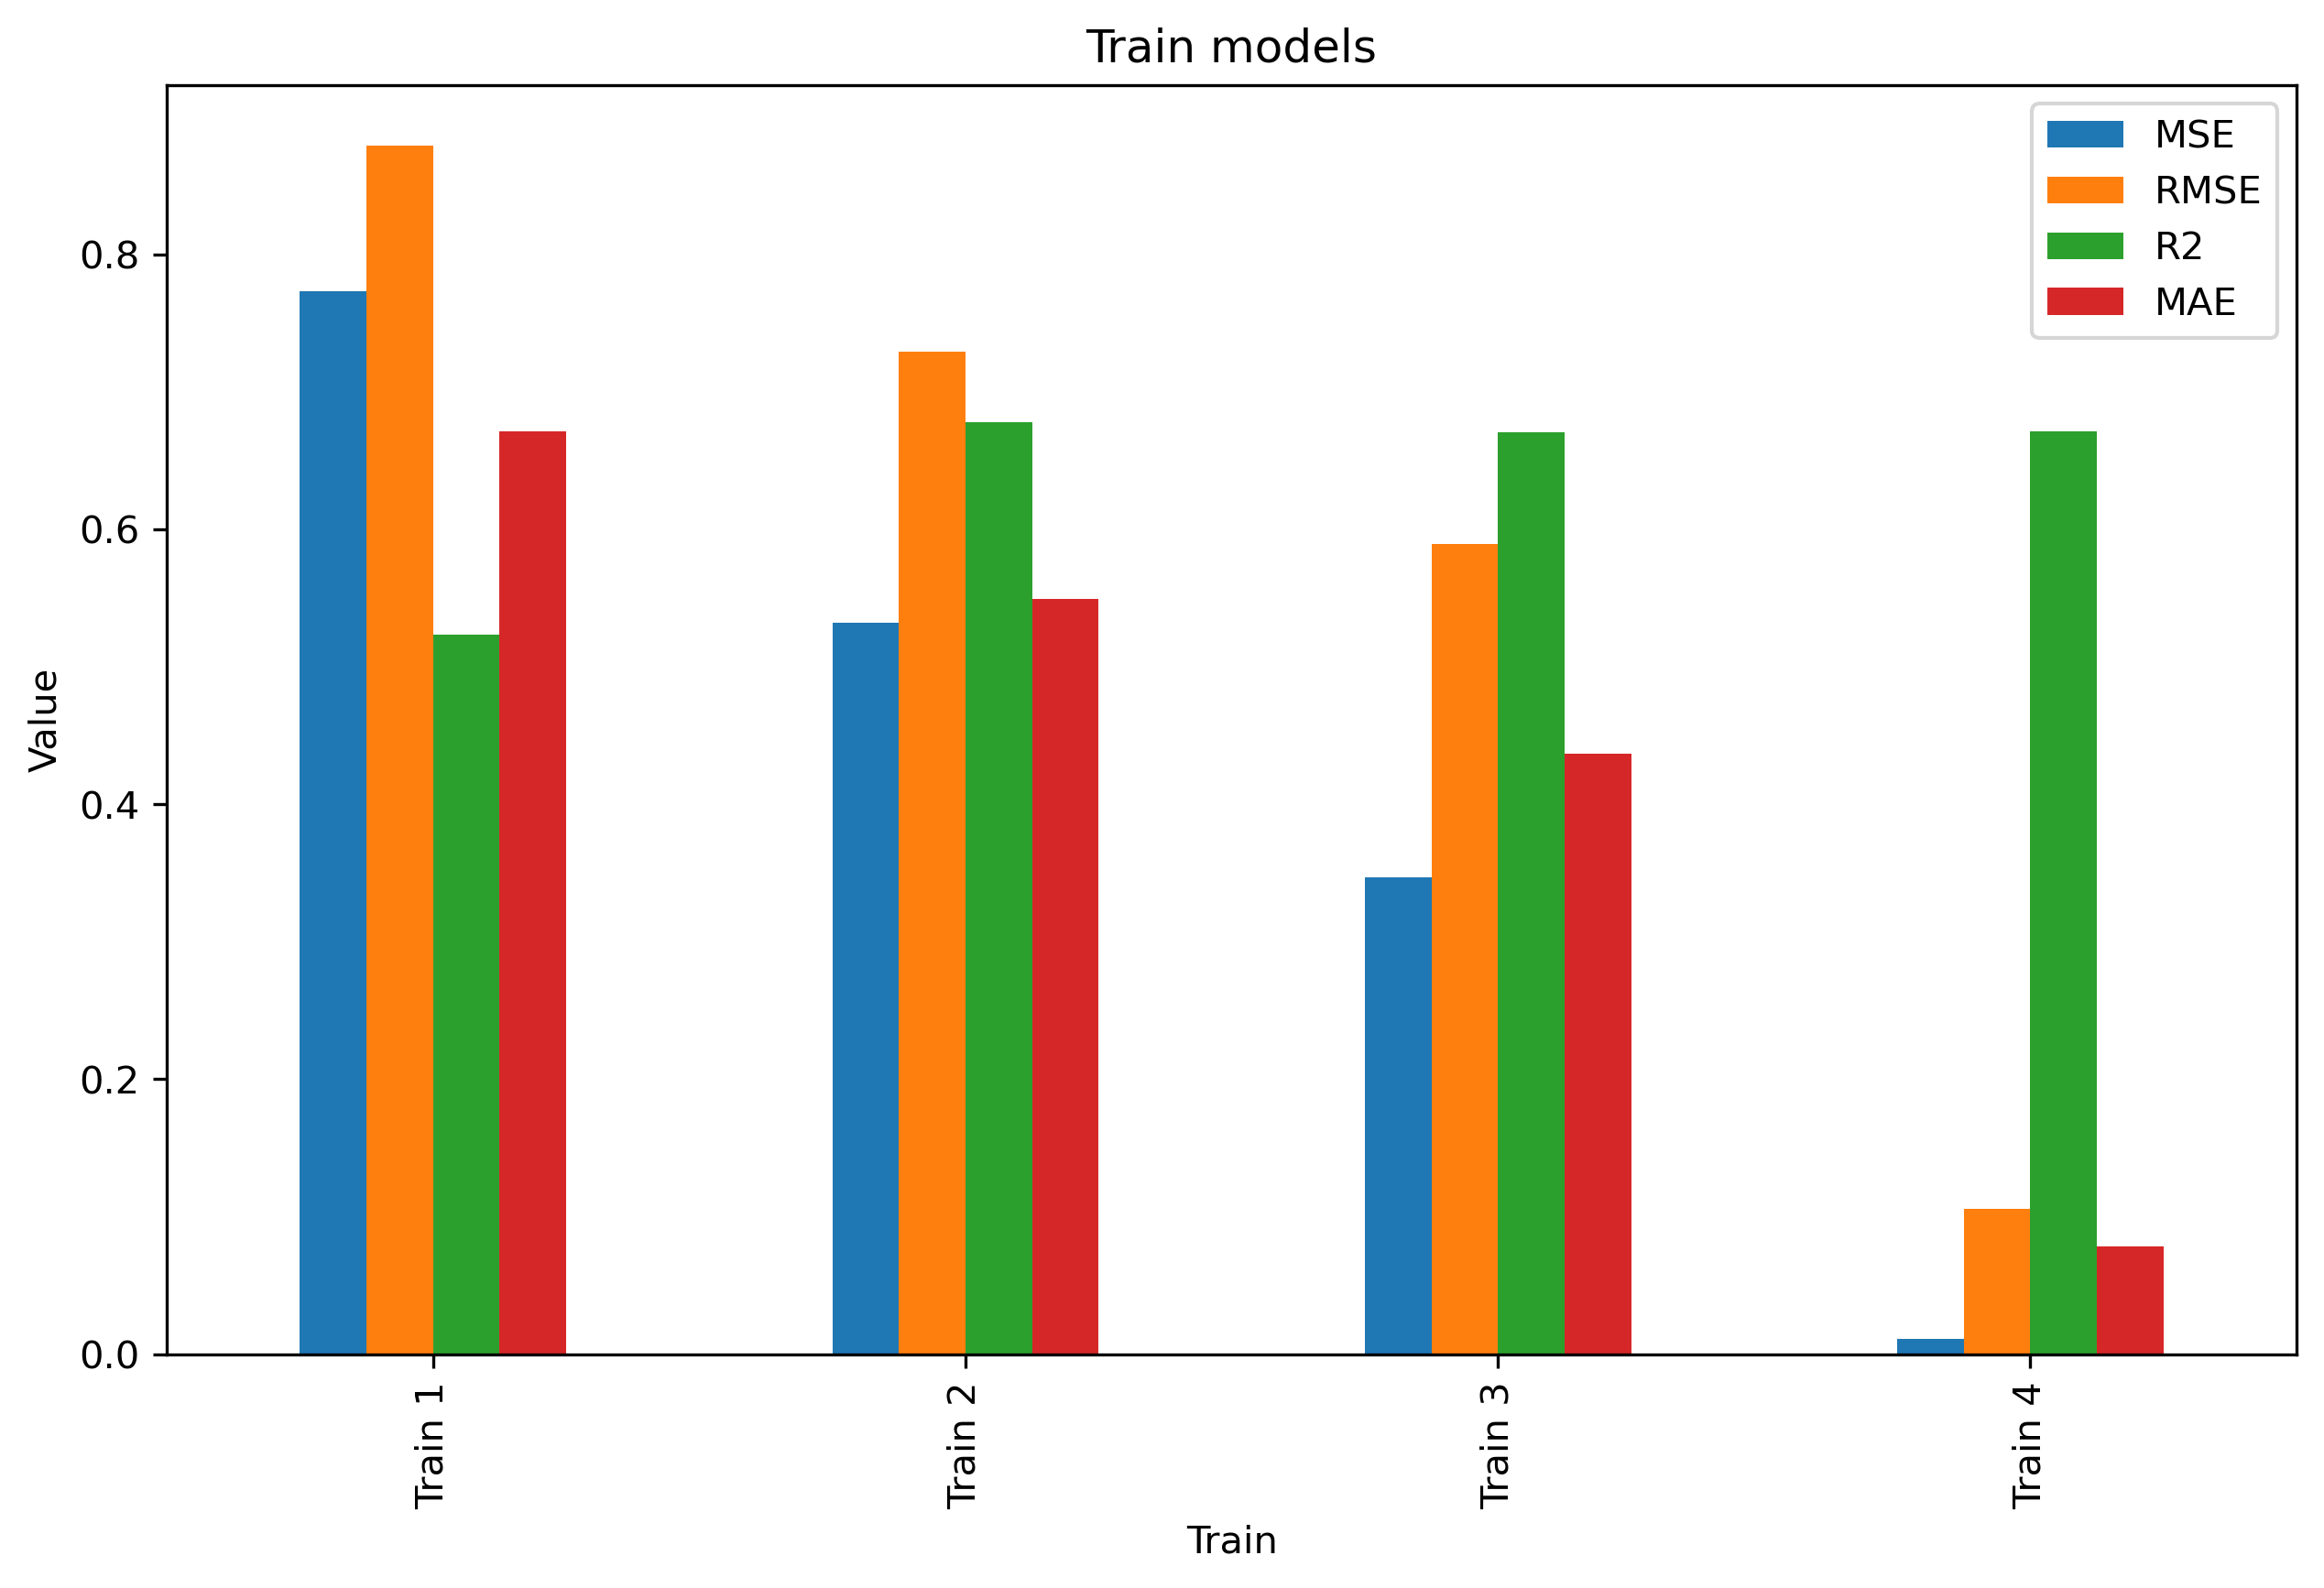
\includegraphics[width=0.4\textwidth]{bar_results_train.png}	
      \caption{Barplot of training set results metrics} 
      \label{Figure5}
  \end{figure}

Once the model predictions have been made, the results of the 200 molecules used for training, for which we already had information about inhibitory activity, were compared with the same 200 molecules resulting from the prediction. In the case of these ones, the algorithm generates a prediction of the activity because when inputting the dataset into the model for prediction, this information was not included. 

When analyzing the results of the histogram (Figure~\ref{Figure6}), it is noted that the distribution of the data is not perfect. Although the figure could suggest a pattern that indicate a good distribution, there are many intermediate values that generate multiple peaks that don't follow the same trend. This can also be observed with the regression line (Figure~\ref{Figure7}), which does not fit the central line of the actual values, indicating that it does not fully adapt to the real values. Furthermore, it can be observed how this dispersion in the distribution increases with higher values. 

\begin{figure}[ht]
    \centering 
     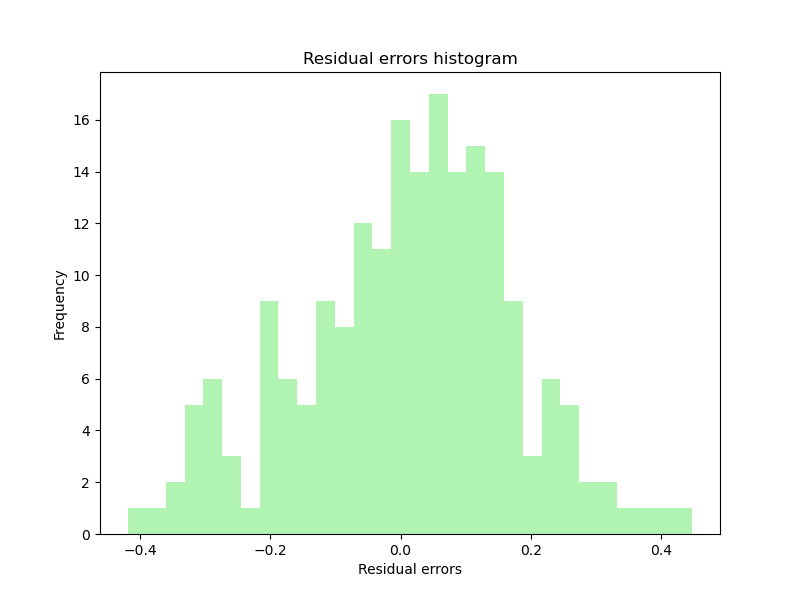
\includegraphics[width=0.4\textwidth]{residual_error_predict_chemdiv.png}	
     \caption{Histogram of predicted residual errors} 
     \label{Figure6}
 \end{figure}

 \begin{figure}[ht]
    \centering 
     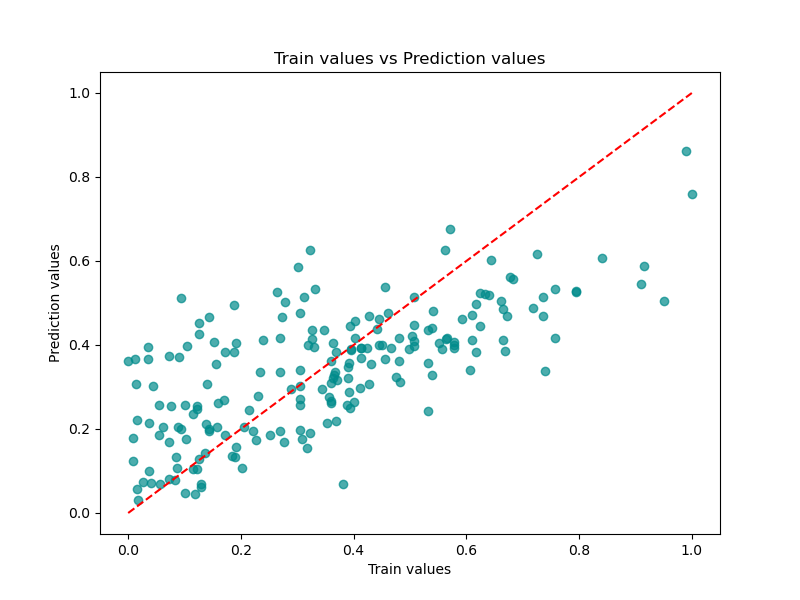
\includegraphics[width=0.4\textwidth]{linregresion_predict_chemdiv.png}	
     \caption{Linear regression of predicted residual errors} 
     \label{Figure7}
 \end{figure}

 To analyze the results obtained from the prediction, correlation graphs between variables have been generated, as well as correlation graphs for each of the calculated variables with the inhibitory activity value. In order to compare these results and draw a conclusion based on real data, the same analysis has also been performed on the data used to train the model used for the predictions. These graphs will provide us information about patterns of data correlation, considering that a value of 1 will indicate a perfect positive correlation between variables, and a value -1 a perfect negative correlation, meaning that when one variable increases, the other decreases. 

 First of all, to analyze the dataset used to train the model (ChEMBL database), we can observe in Figure~\ref{Figure8} that the variables most correlated with each other are Molecular Weight (MW) with Heavy Atom Counts and Hydrogen Bond Donor (H-bond donor) with Topological Polar Surface Area (TPSA) with correlation values of 0,99 and 0,82 respectively. Looking at Figure~\ref{Figure9}, we see that the maximum correlation value is 0,13. This indicates that, in general, the correlation of the variables with what interests us is not very high. The variables most correlated with the value of inhibitory activity within the given values, are Rotatable Bonds, with a value of 0,13, and Balaban J Index, with a value of 0,11. 

\begin{figure}[h]
    \begin{subfigure}{0.5\textwidth}
        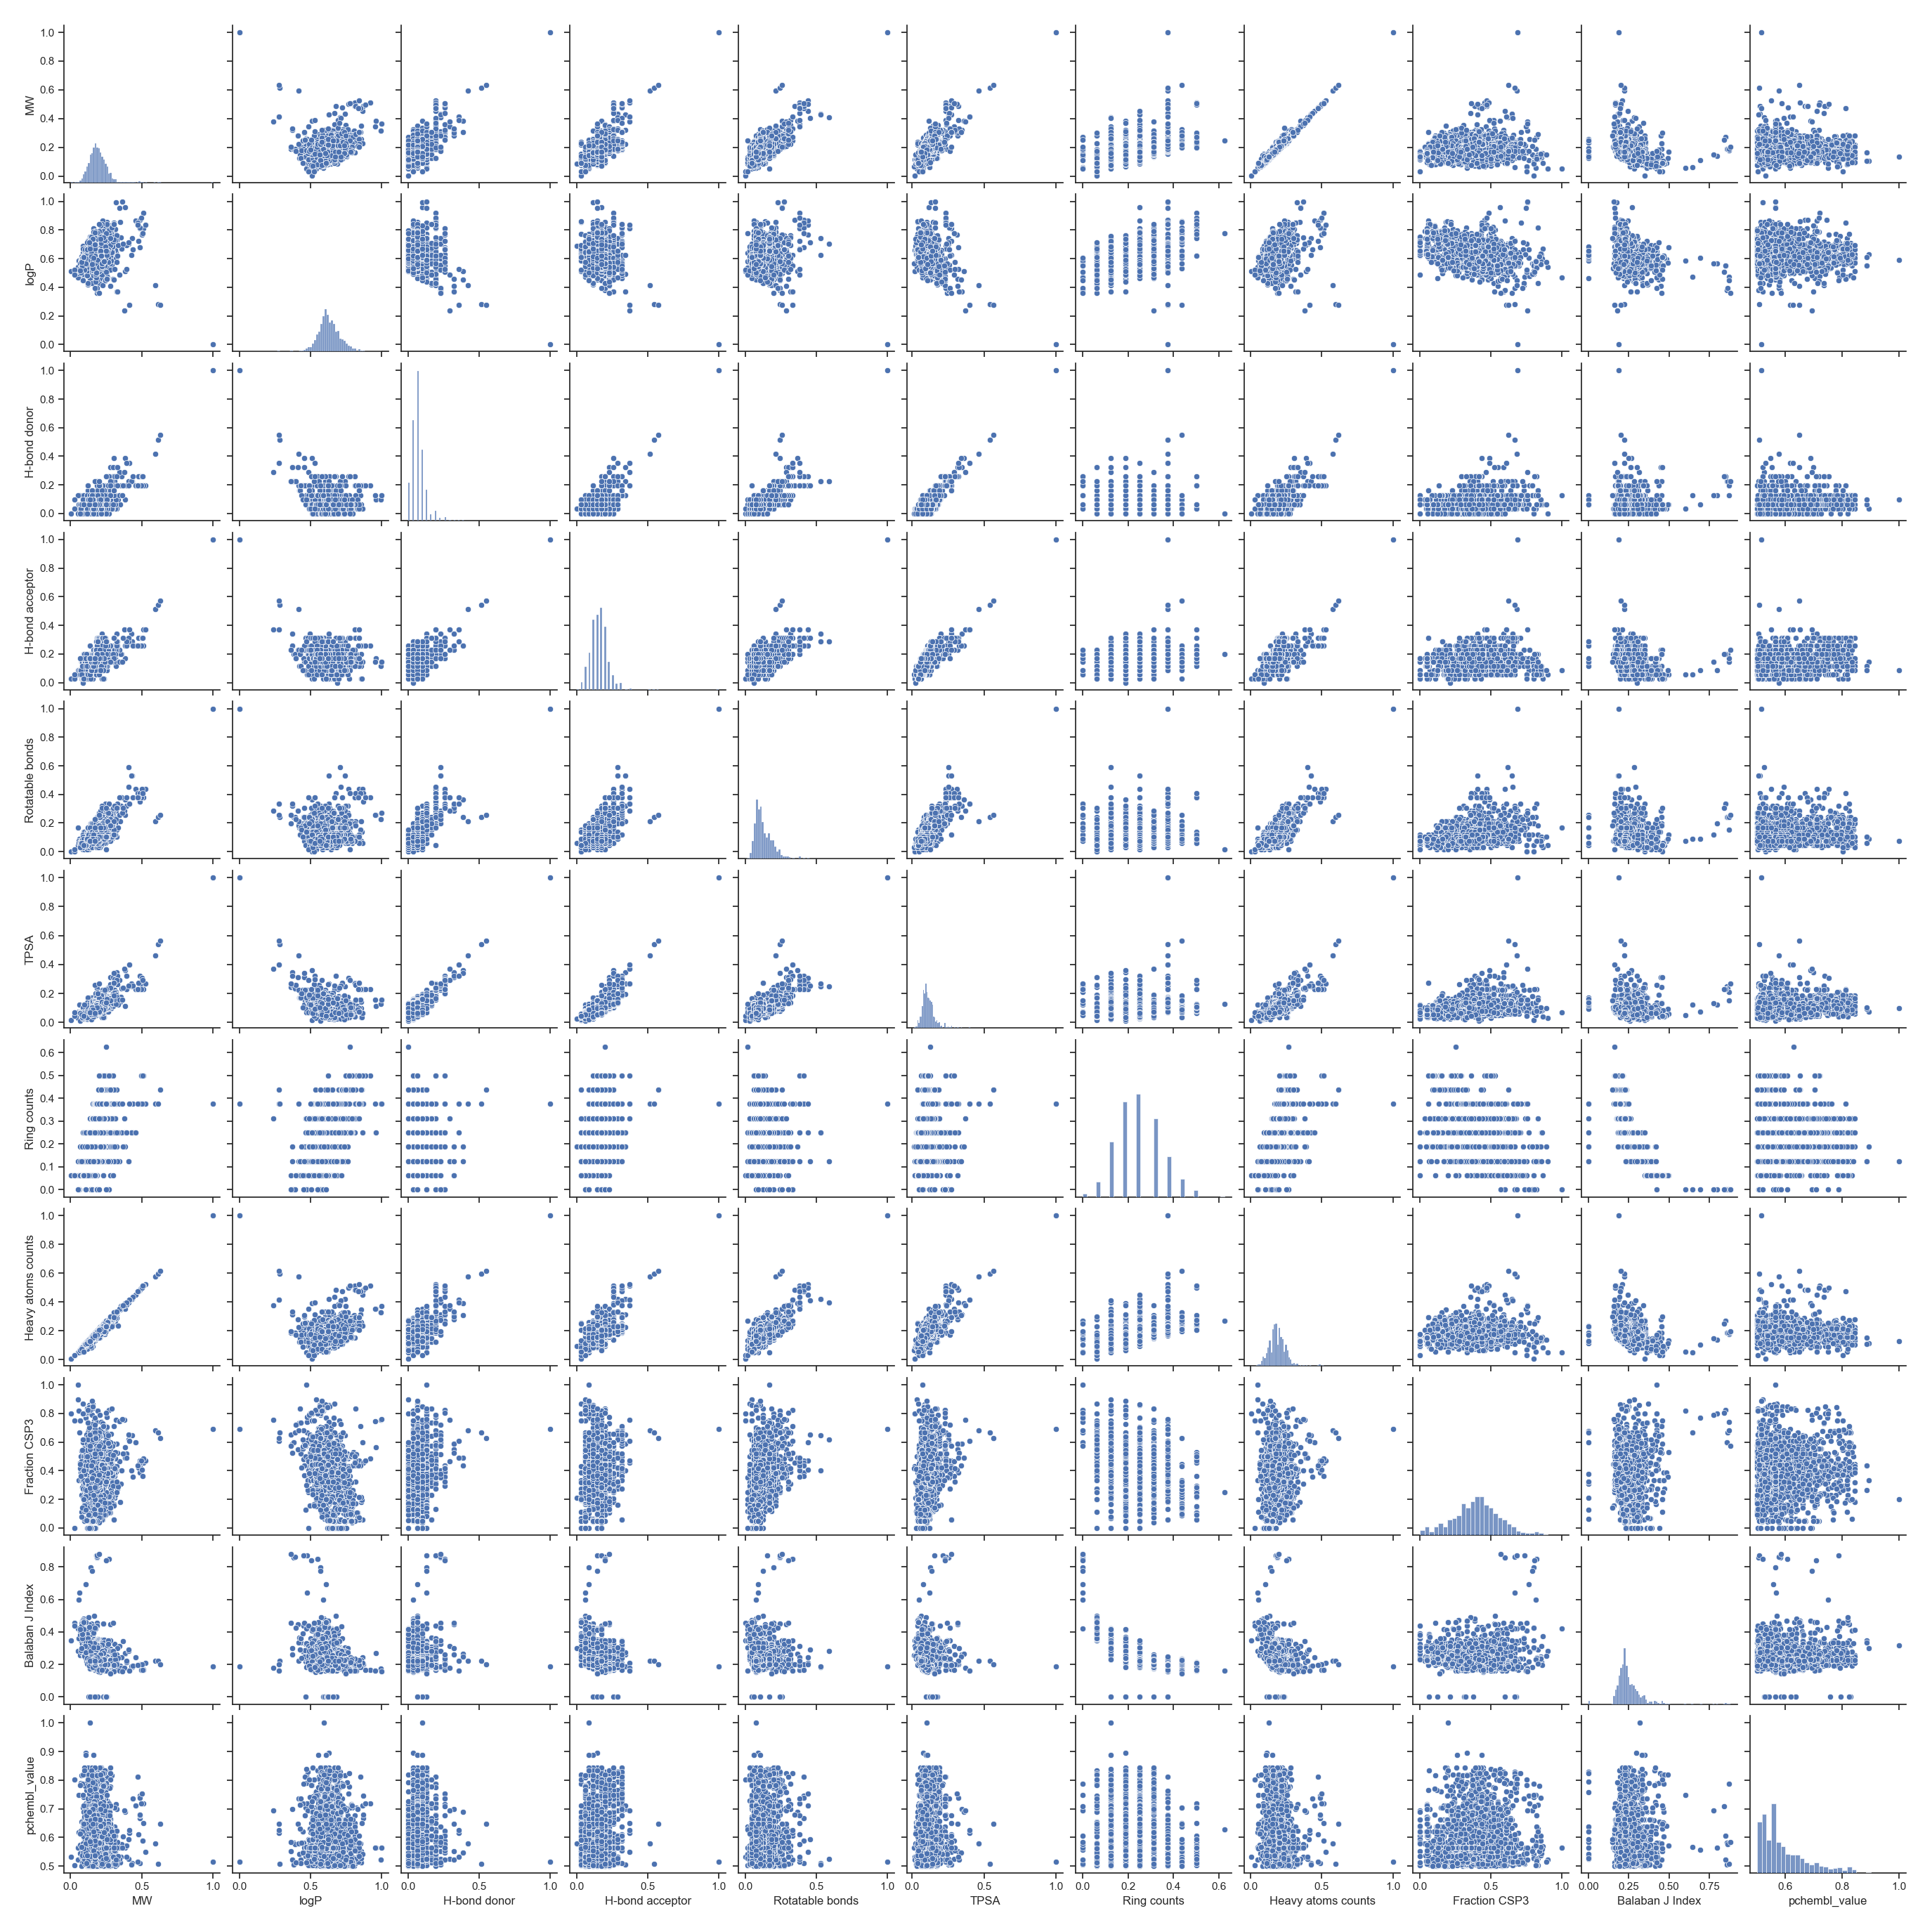
\includegraphics[width=0.8\linewidth, height=4cm]{pairplot_matrix_train4.png} 
        \caption{}%%Pairplot correlation matrix
        %%\label{fig:subim1}
    \end{subfigure}
    \hfill
    \begin{subfigure}{0.5\textwidth}
        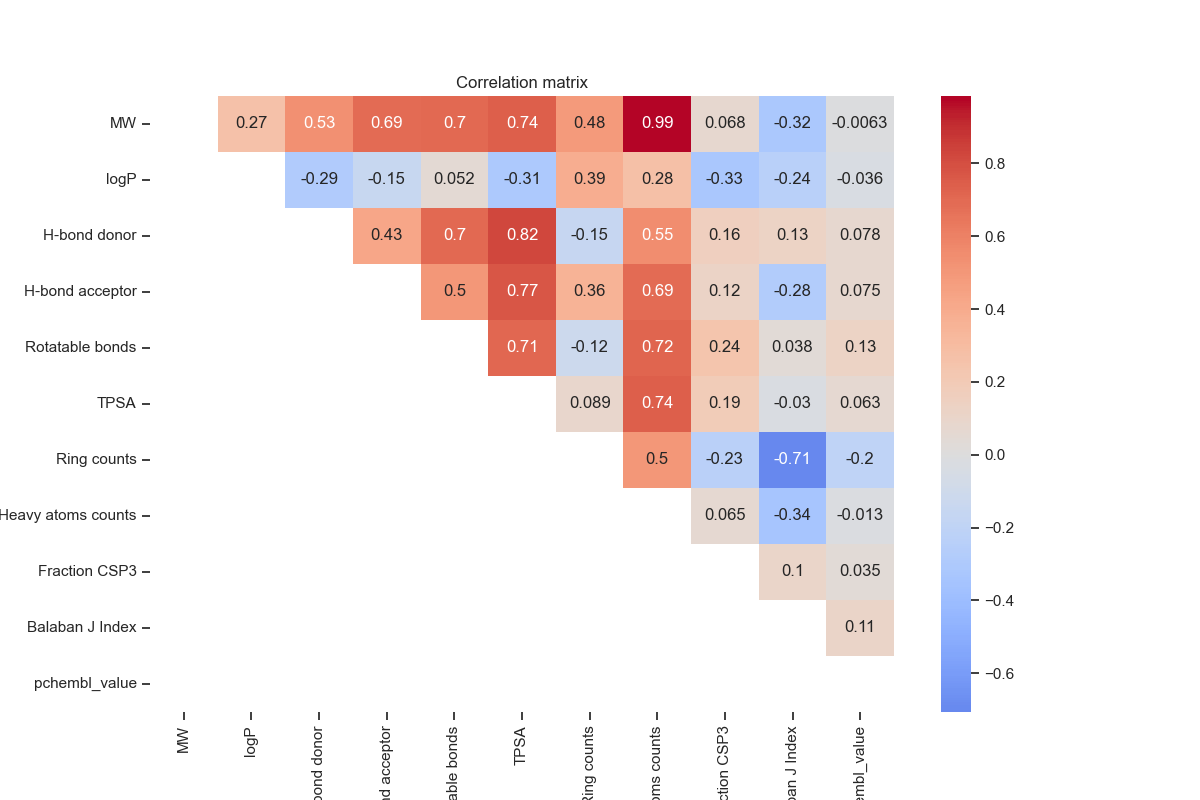
\includegraphics[width=0.8\linewidth, height=4cm]{migheatmap_train4.png}
        \caption{} %%Correlation matrix
        %%\label{fig:subim2}
    \end{subfigure}
    
    \caption{Correlation analysis from the dataset used to train the model (ChEMBL). (a) Pariplot correlation matrix. (b)Correlation matrix heatmap}
    \label{Figure8}
\end{figure}

\begin{figure}[h]
    \centering 
     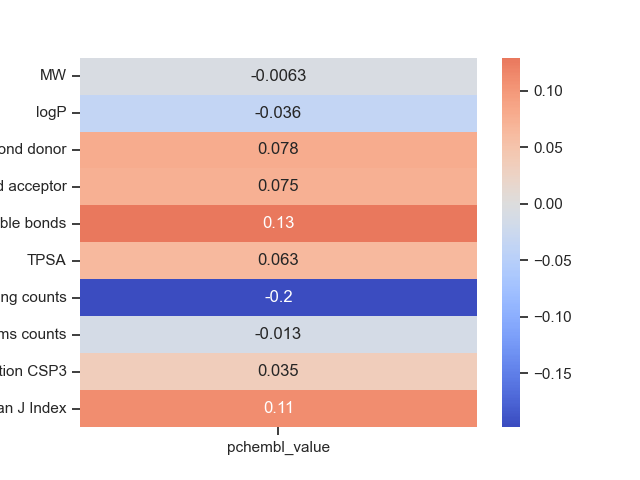
\includegraphics[width=0.4\textwidth]{cor_plot3_pchembl_train4.png}	
     \caption{Correlation heatmap of variables with the -log(molar IC50) value from the dataset used to train the model} 
     \label{Figure9}
 \end{figure}

 The results for the dataset of the first prediction (ChemDiv database), show that the most correlated variables among them, as see in Figure~\ref{Figure10}, are MW with Heavy Atom Counts, H-bond Donor with Rotatable Bonds and H-bond Acceptor with TPSA, with correlation values of 0,97 , 0,85 and 0,85 respectively. Regarding the relationship of each variable with the activity value (Figure~\ref{Figure11}), the ones with the highest correlation are H-bond acceptor and Rotatable Bonds with correlation values of 0,34 and 0,3. 

 For the dataset of the second train (Zinc database), the variables most related to each other, as seen in Figure~\ref{Figure13}, are MW with Heavy Atom Counts and TPSA with Heavy Atom Counts, with correlation values of 0,98 and 0,9 respectively. The variables that are most related to the activity value (Figure~\ref{Figure12}) are H-bond acceptor and TPSA with values 0,41 and 0,34. 

\begin{figure}[h]
    \begin{subfigure}{0.5\textwidth}
        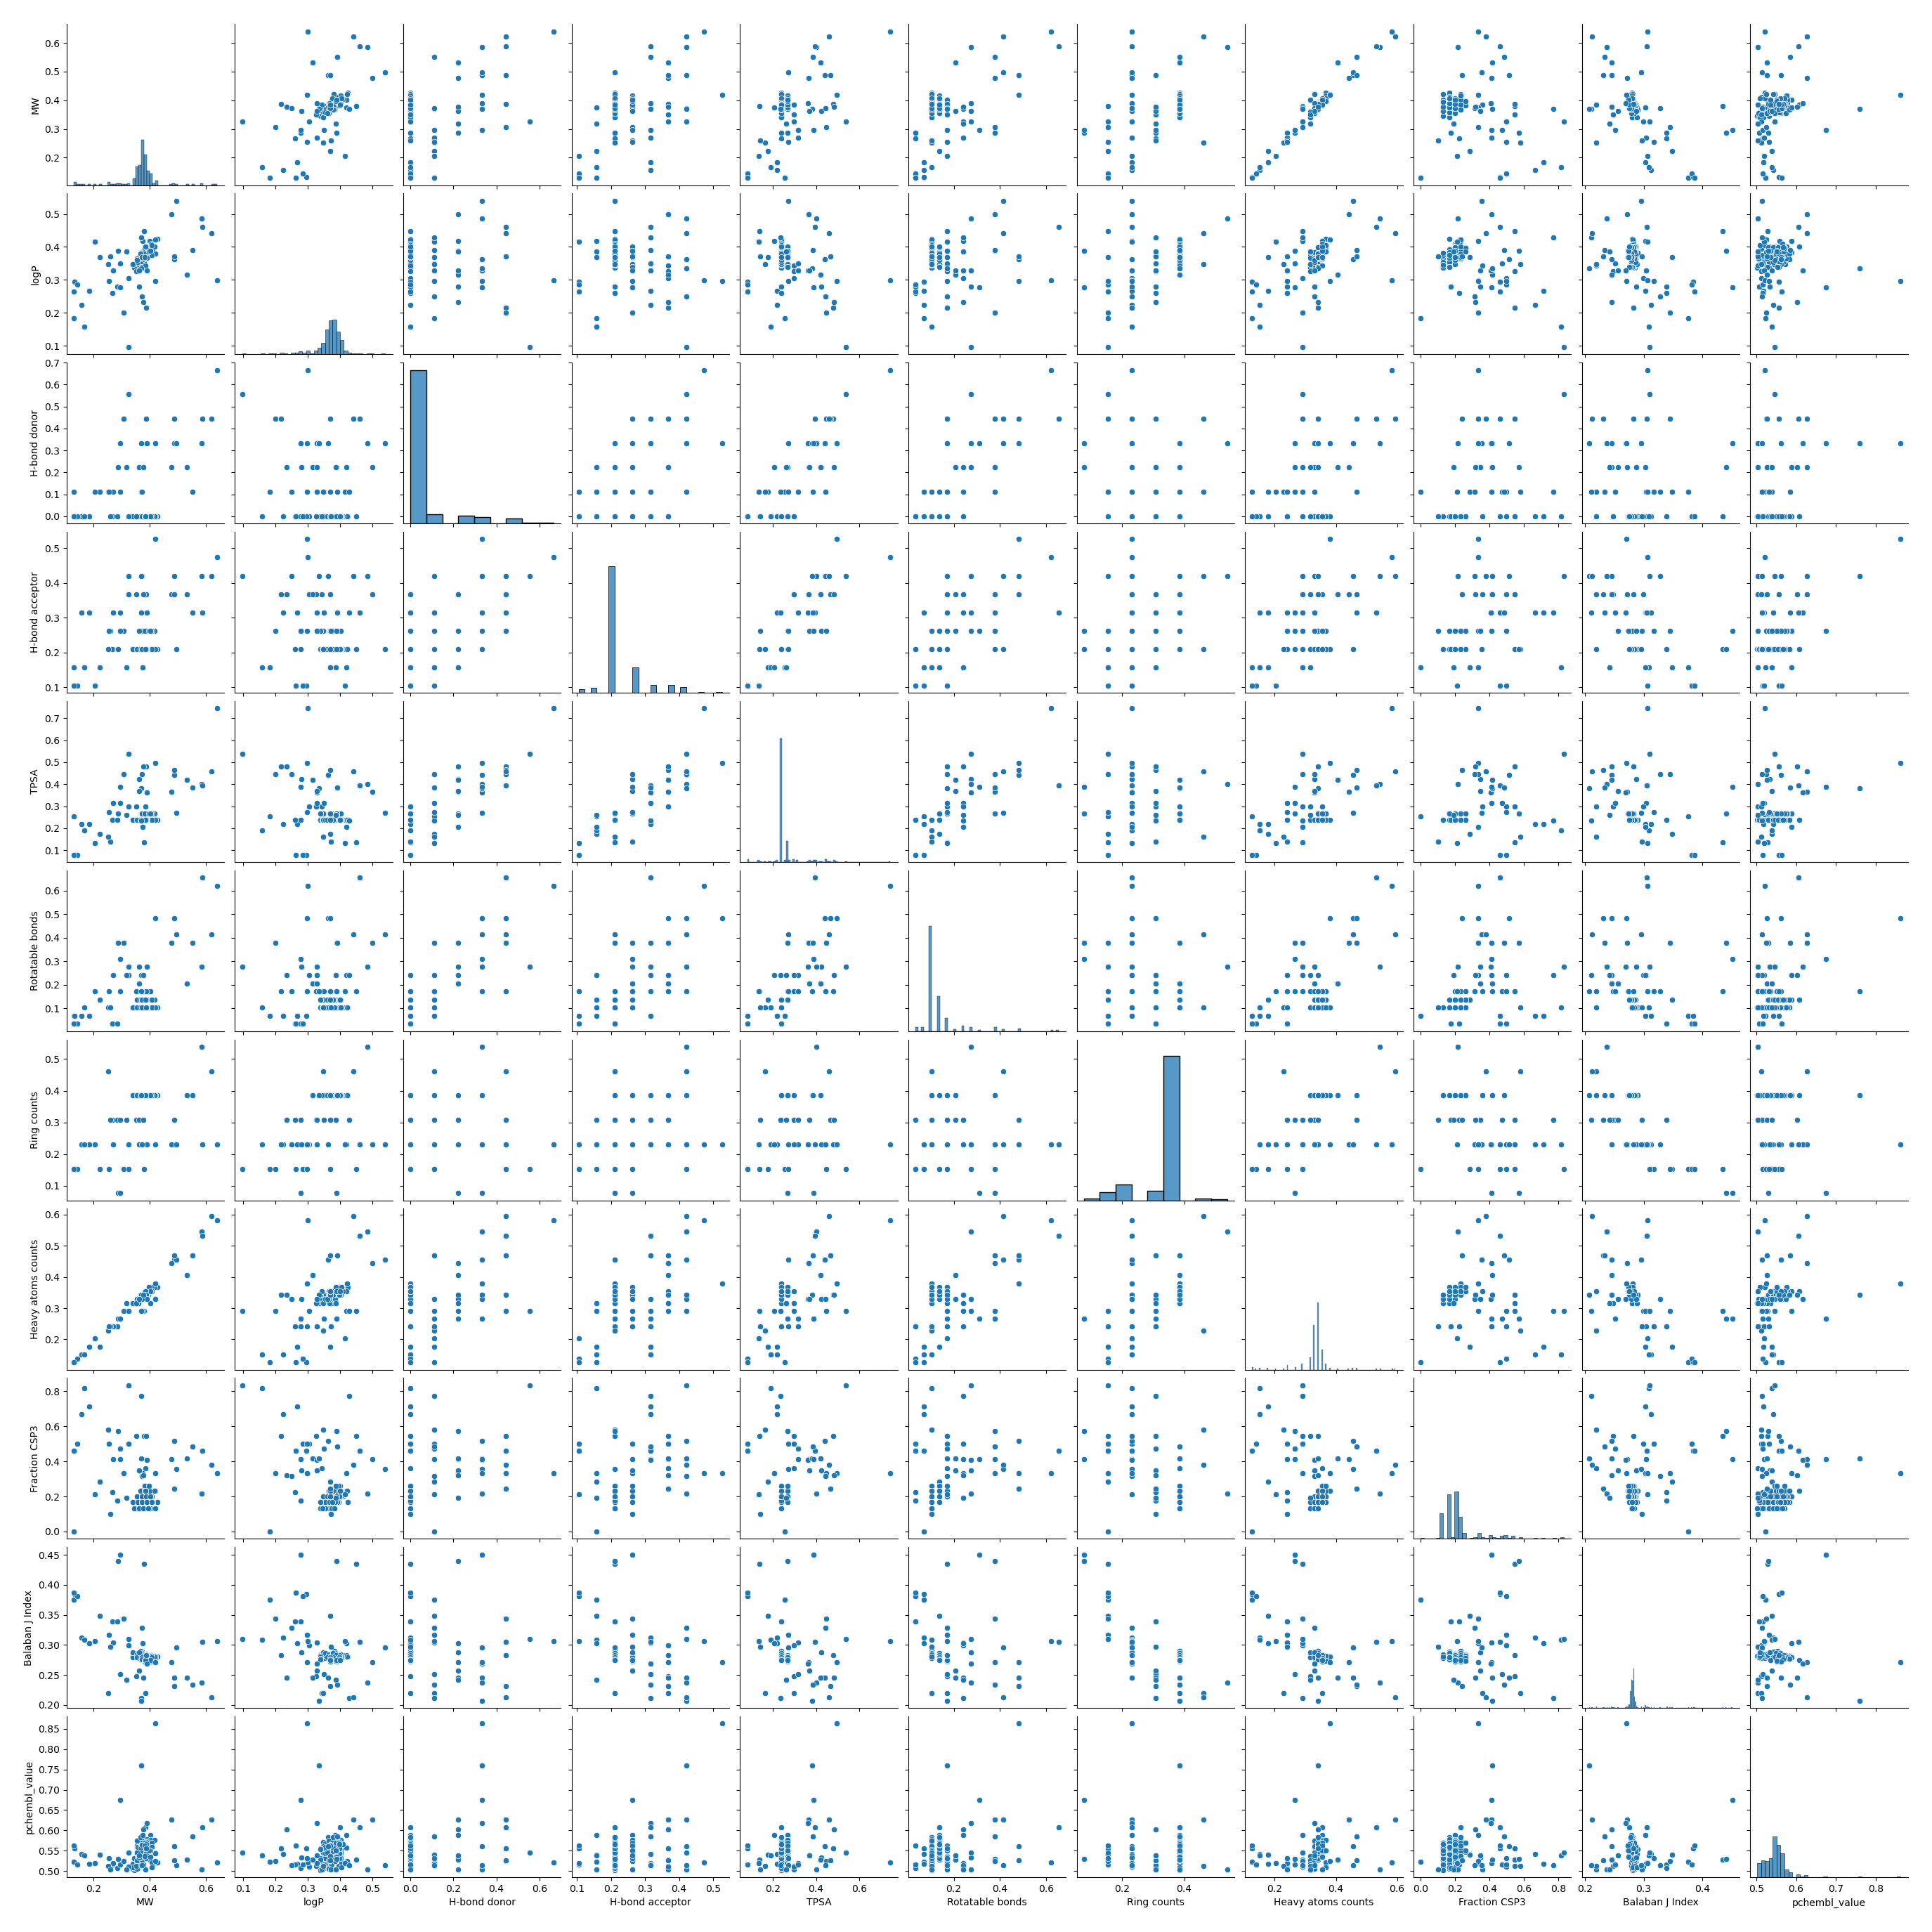
\includegraphics[width=0.8\linewidth, height=4cm]{pairplot_matrix_predict_chemdiv.png} 
        \caption{Pairplot correlation matrix}
        %%\label{fig:subim1}
    \end{subfigure}
    \begin{subfigure}{0.5\textwidth}
        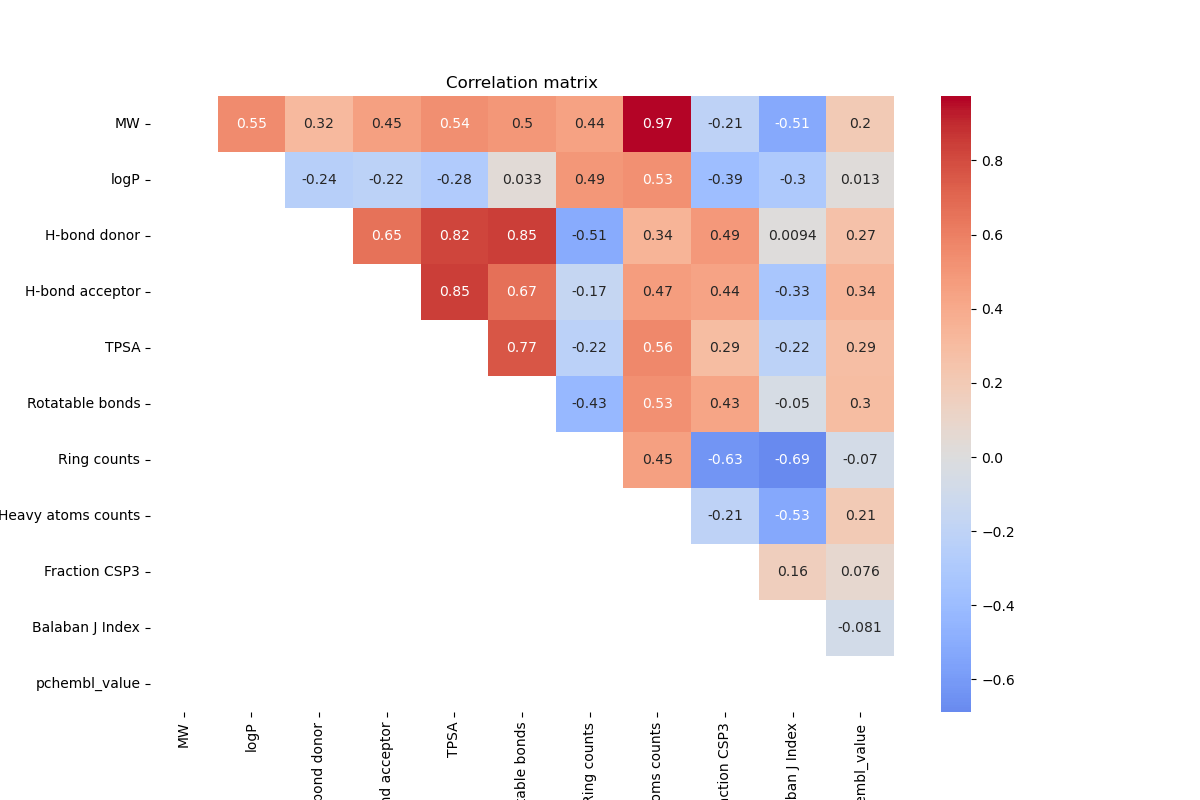
\includegraphics[width=0.8\linewidth, height=4cm]{migheatmap_predict_chemdiv.png}
        \caption{Correlation matrix}
        %%\label{Figure8}
    \end{subfigure}
    
    \caption{Correlation analysis from the dataset used to the first predict model (ChemDiv). (a)Pariplot correlation matrix (b)Correlation matrix heatmap}
    \label{Figure10}
\end{figure}

\begin{figure}[h]
    \centering 
     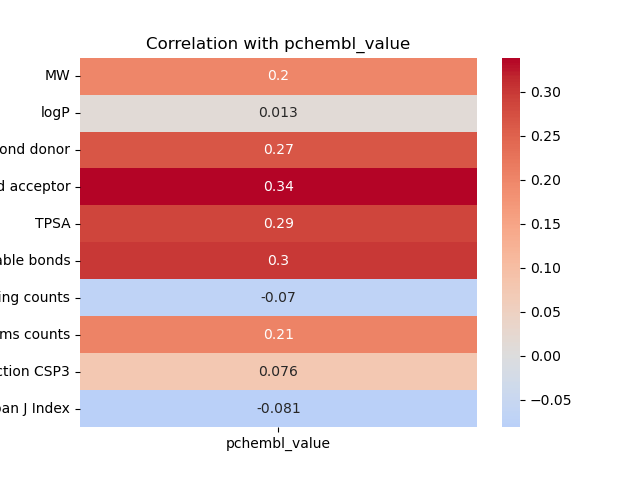
\includegraphics[width=0.4\textwidth]{cor_plot3_pchembl_predict_chemdiv.png}	
     \caption{Correlation heatmap of variables with the -log(molar IC50) value from the dataset used to the first predict model} 
     \label{Figure11}
 \end{figure}

 \begin{figure}[h]
    \centering 
     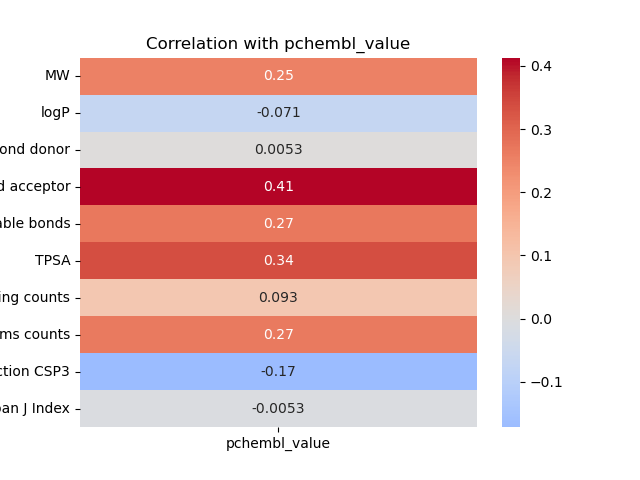
\includegraphics[width=0.4\textwidth]{cor_plot3_pchembl_predict_zinc.png}	
     \caption{Correlation heatmap of variables with the -log(molar IC50) value from the dataset used to the second predict model} 
     \label{Figure12}
 \end{figure}

 \begin{figure}[h]
    \begin{subfigure}{0.5\textwidth}
        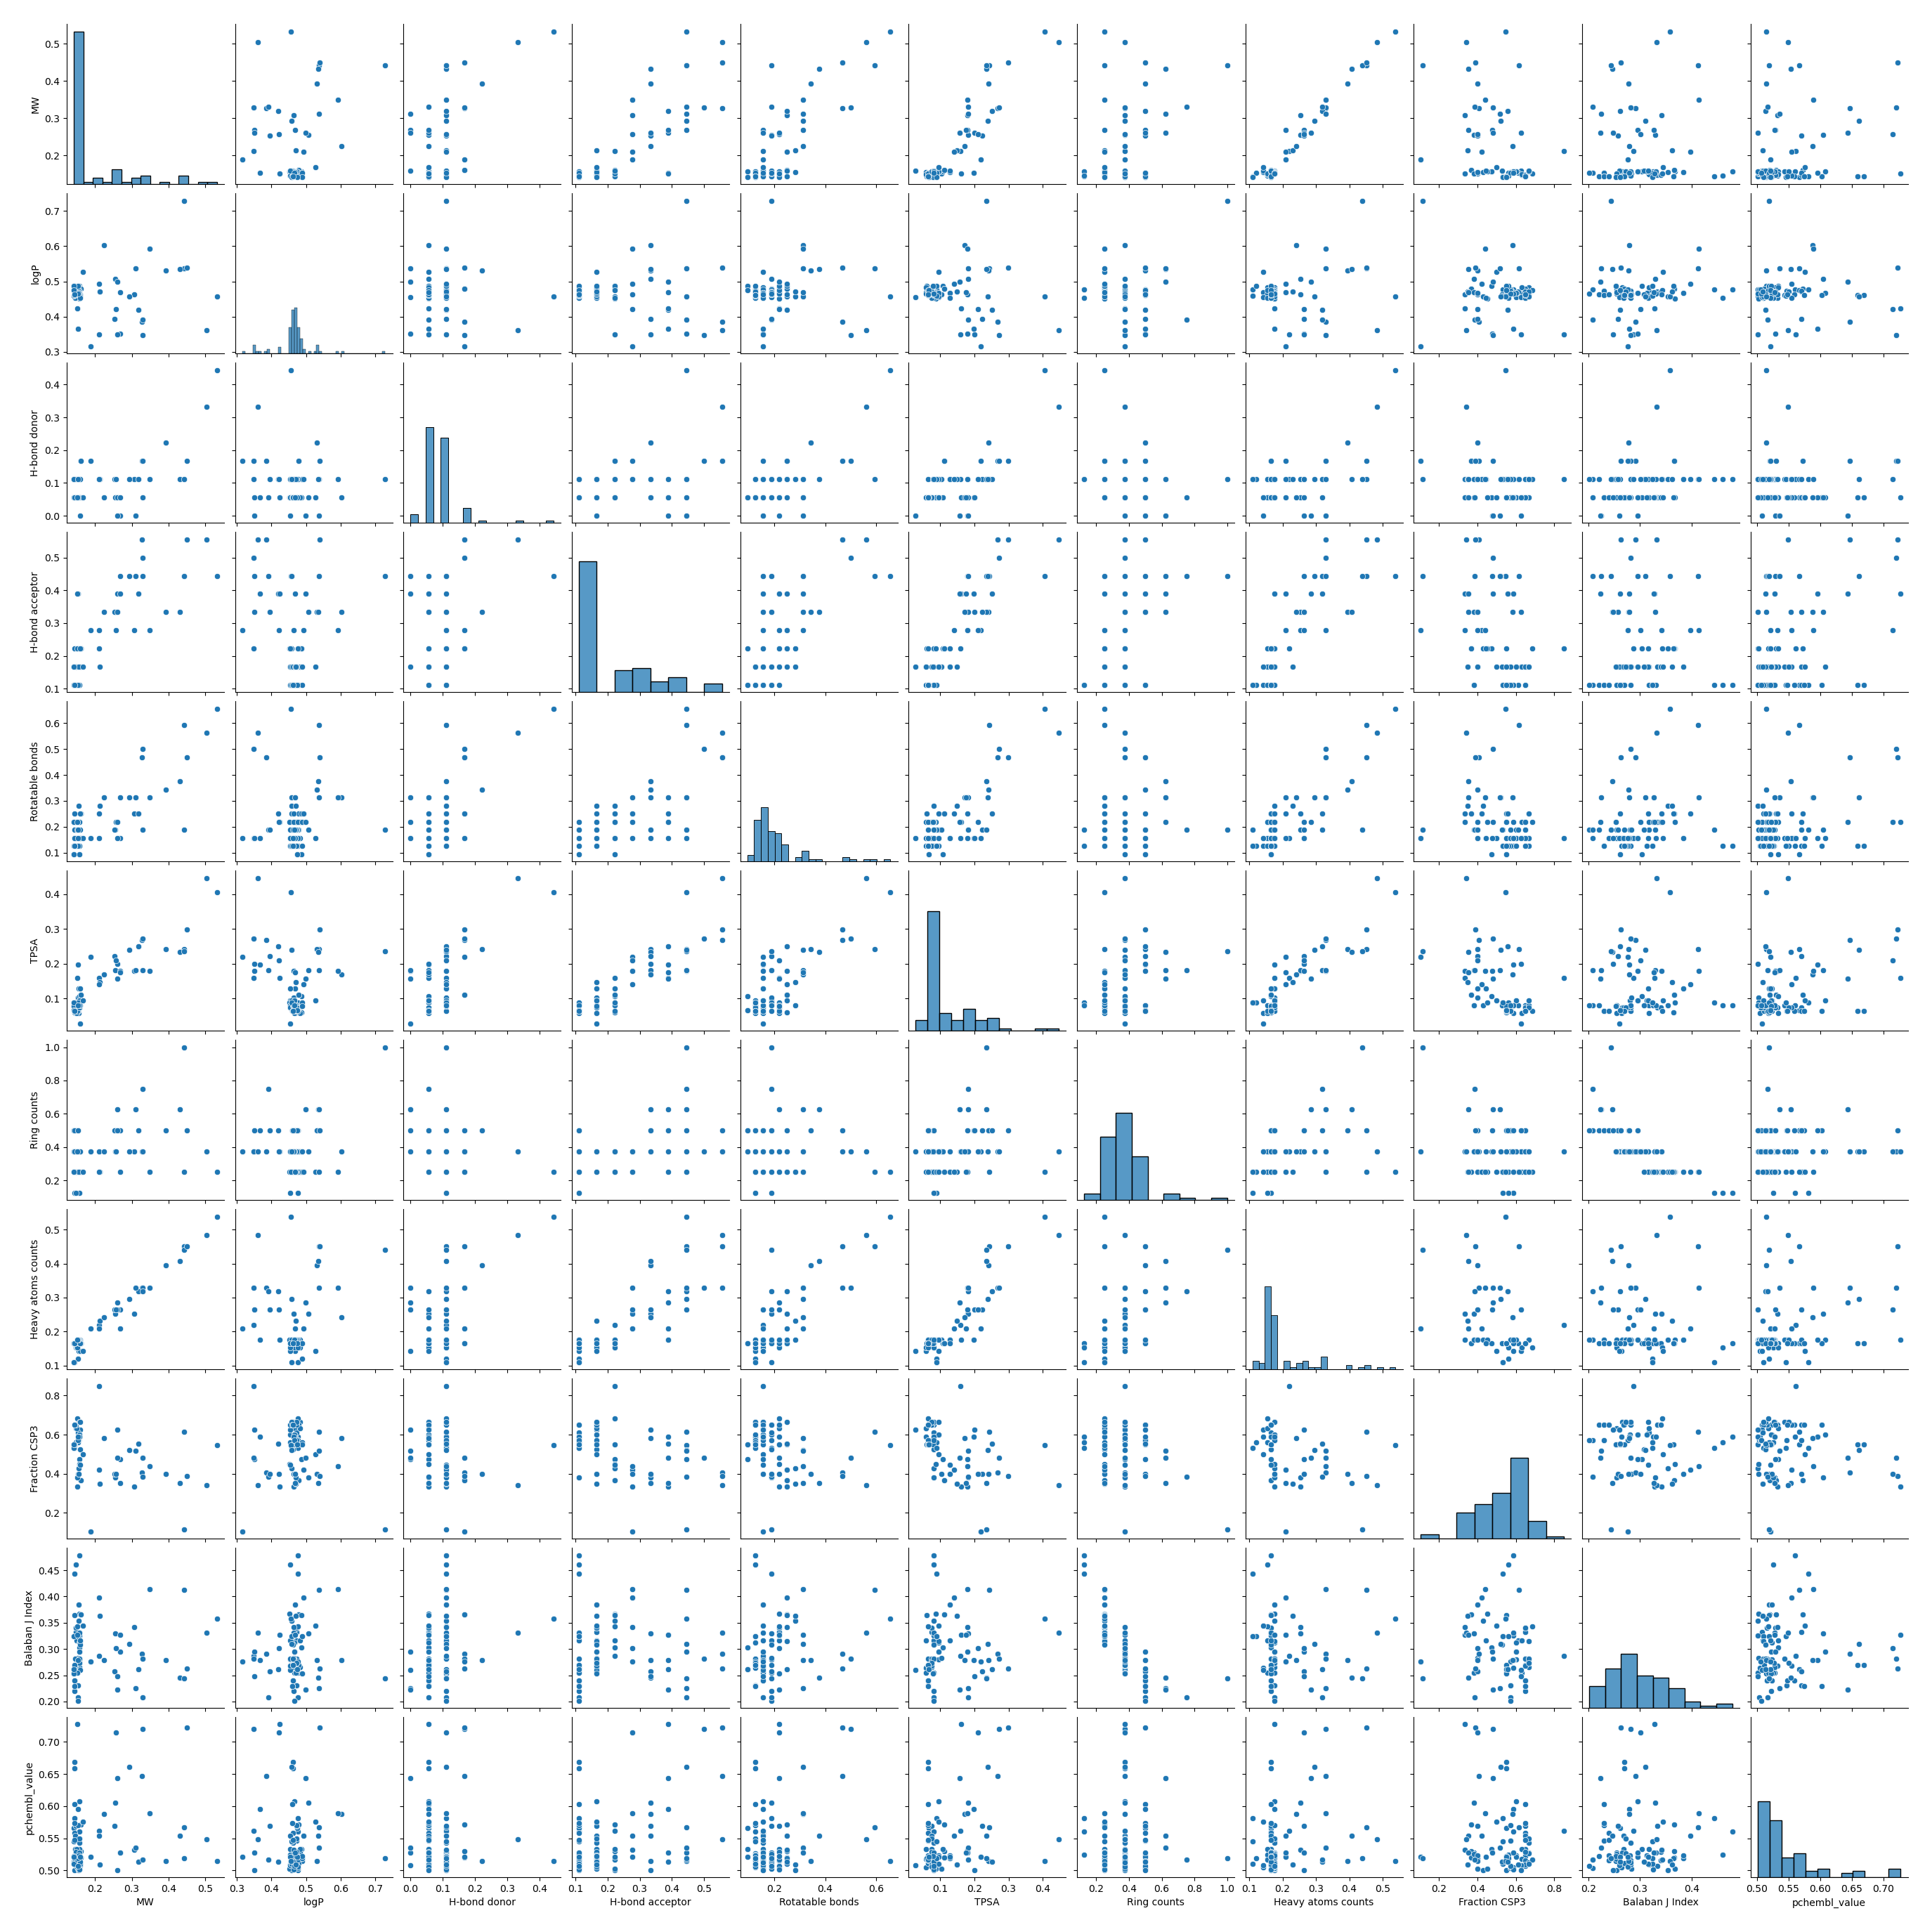
\includegraphics[width=0.9\linewidth, height=6cm]{pairplot_matrix_predict_zinc.png} 
        \caption{Pairplot correlation matrix}
        %%\label{fig:subim1}
    \end{subfigure}
    \begin{subfigure}{0.5\textwidth}
        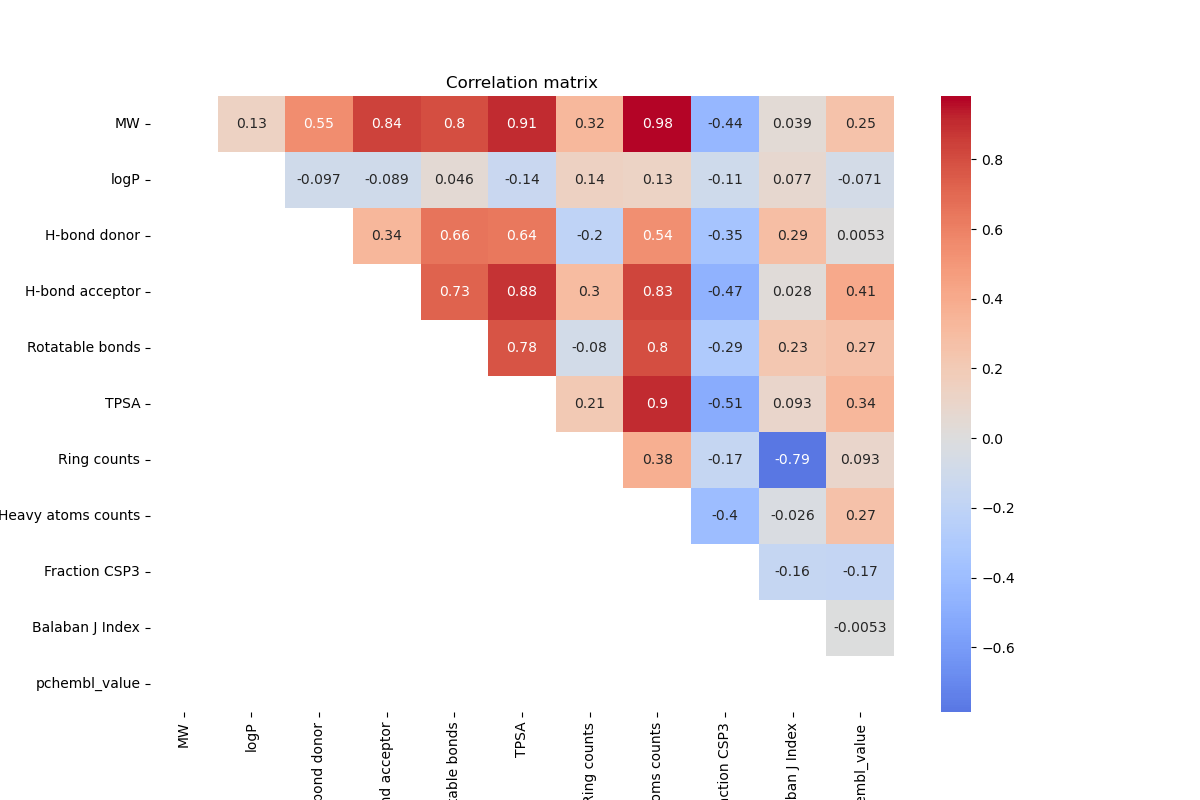
\includegraphics[width=0.9\linewidth, height=6cm]{migheatmap_predict_zinc.png}
        \caption{Correlation matrix}
        %%\label{fig:subim2}
    \end{subfigure}
    
    \caption{Correlation analysis from the dataset used to the second predict model}
    \label{Figure13}
\end{figure}

 %%SIMILARITY
 \begin{figure}[h]
    \centering 
     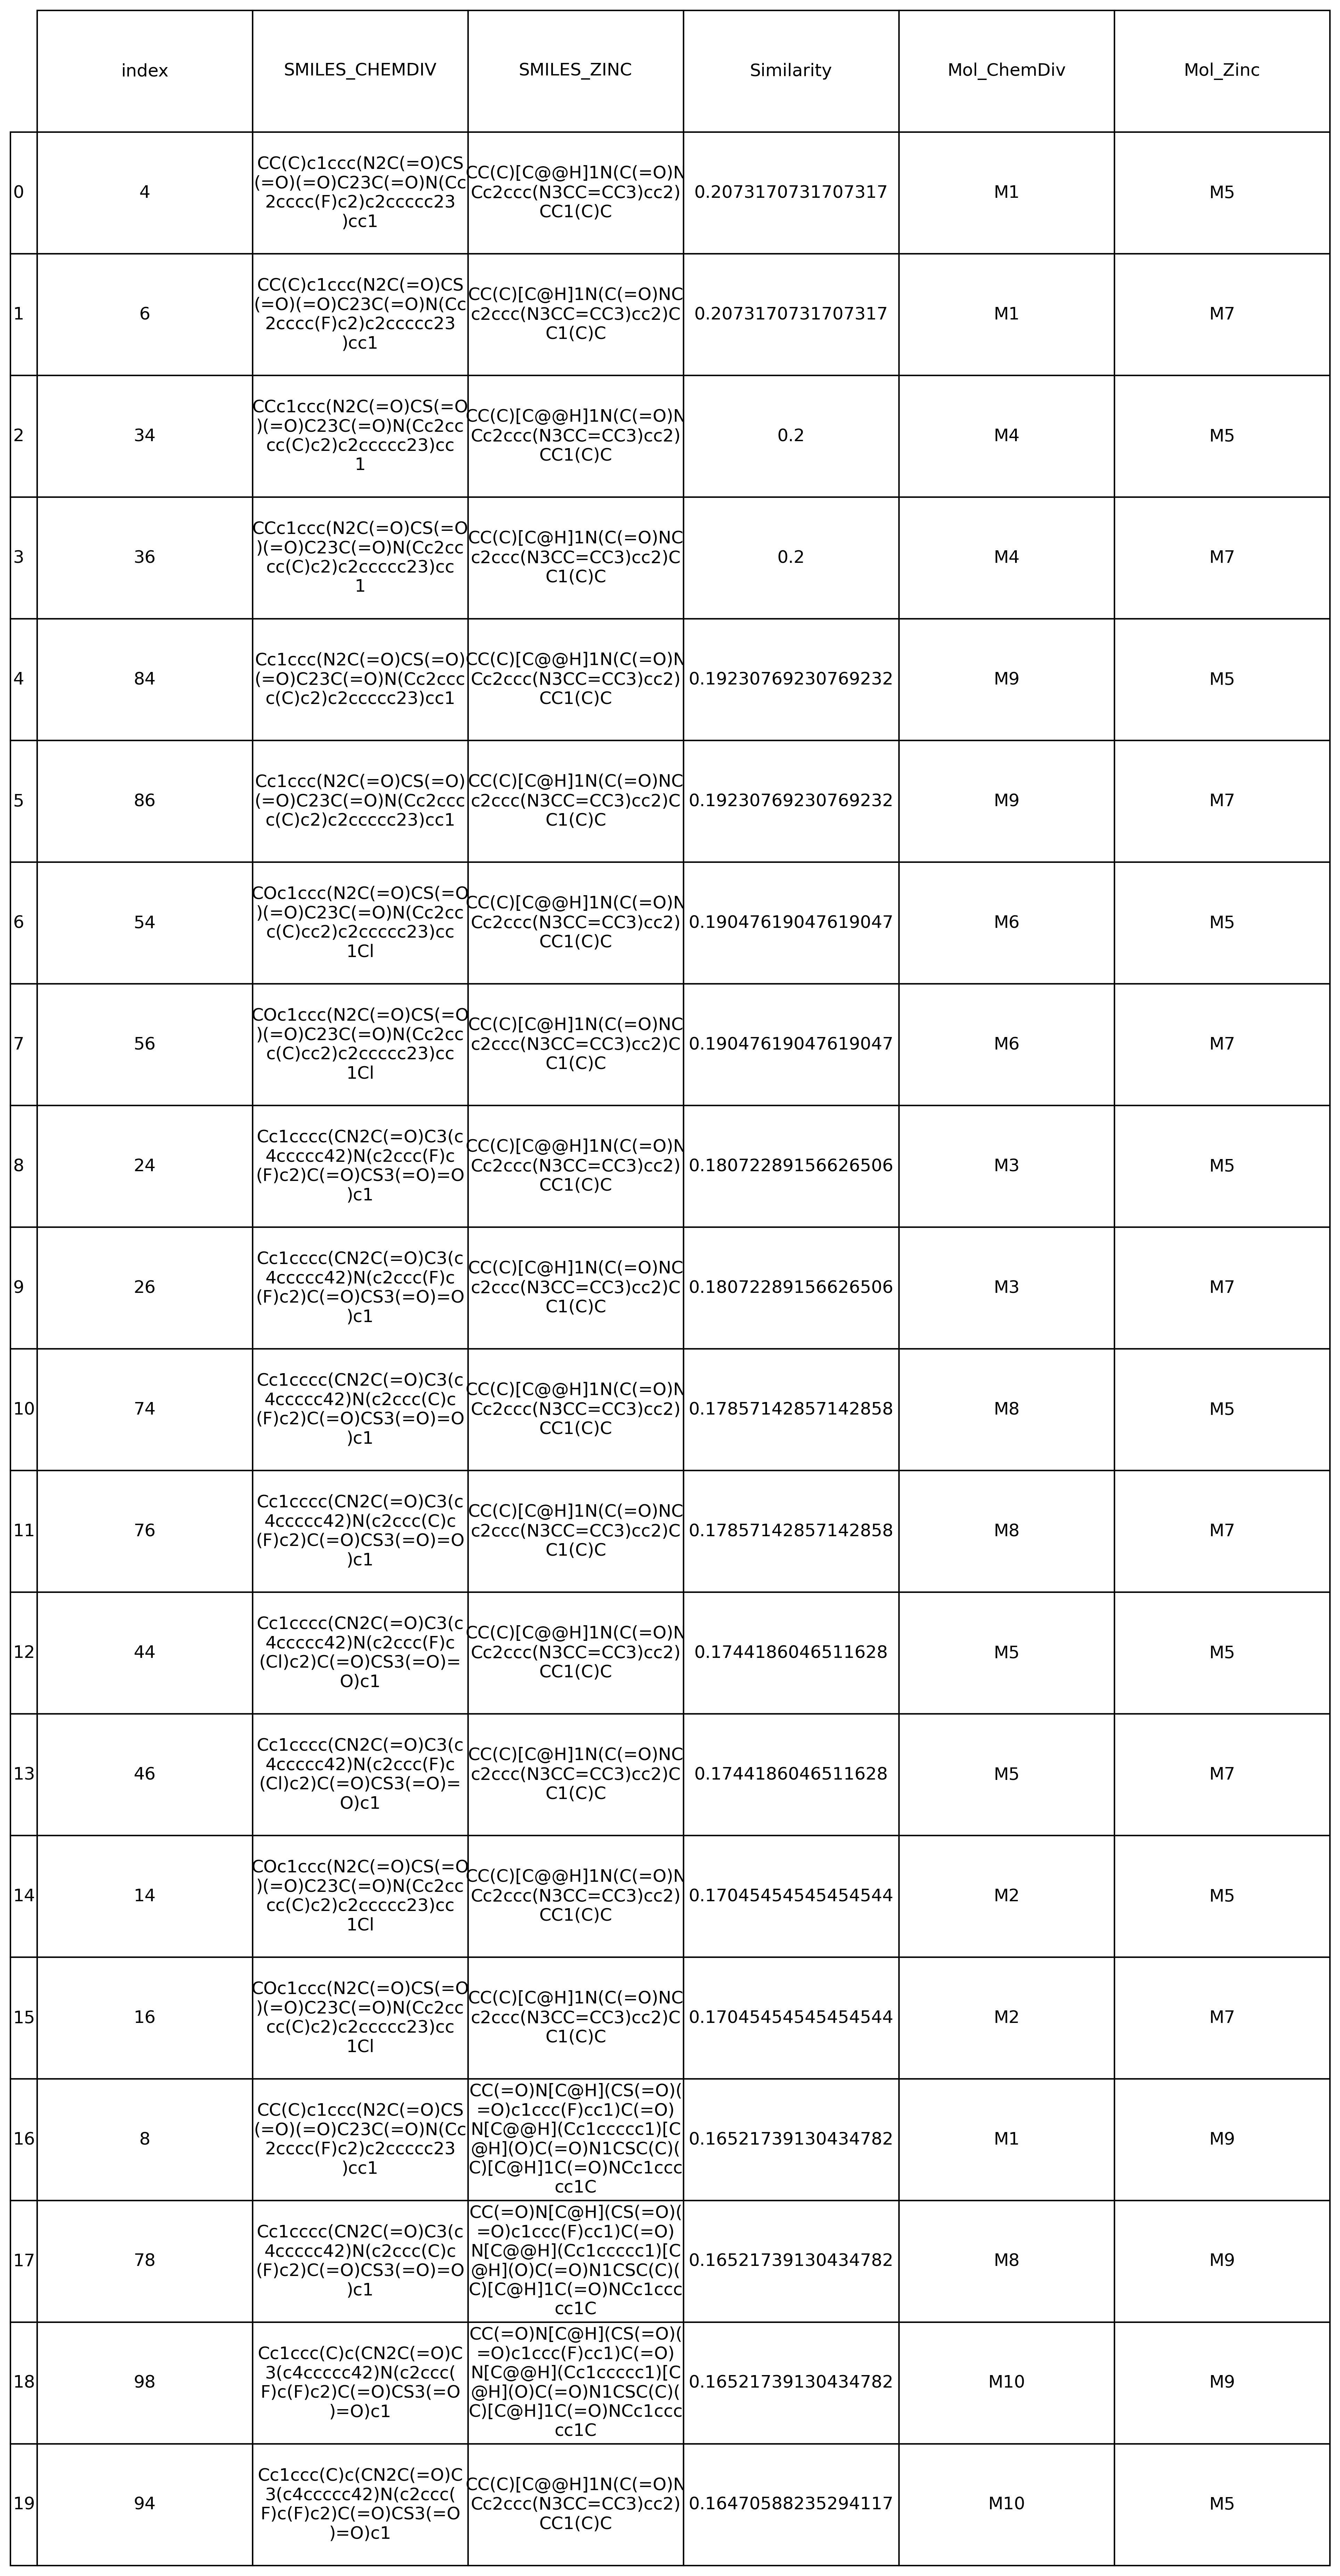
\includegraphics[width=0.4\textwidth]{best_similarity_resultspred.png}	
     \caption{Results from the similarity analysis from the two predicted results.} 
     \label{Figure14}
 \end{figure}

 \begin{figure*}[h]
    \centering 
     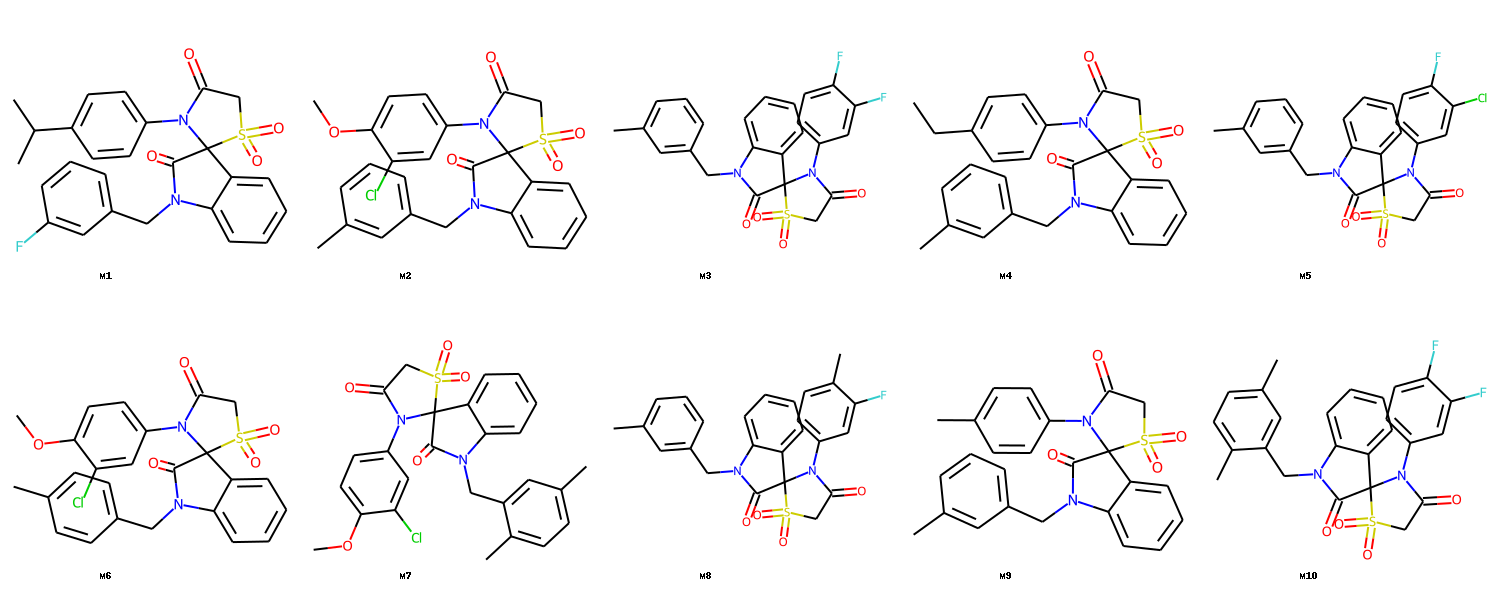
\includegraphics[width=0.4\textwidth]{top10_mol_chemdiv.png}	
     \caption{The 10 molecules from the first predicted results with a higher activity value} 
     \label{Figure15}
 \end{figure*}

 \begin{figure*}[h]
    \centering 
     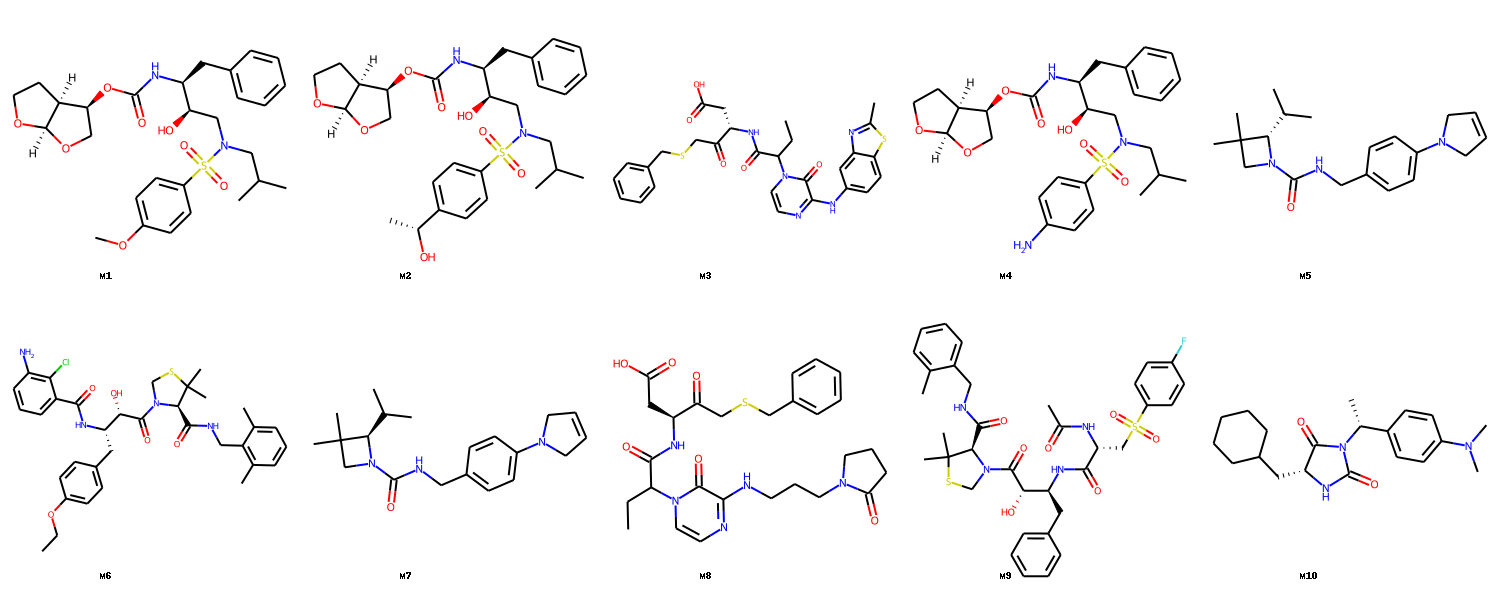
\includegraphics[width=0.4\textwidth]{top10_mol_zinc.png}	
     \caption{The 10 molecules from the second predicted results with a higher activity value} 
     \label{Figure16}
 \end{figure*}

 \begin{figure*}[h]
    \centering
    \begin{subfigure}{0.9\textwidth}
        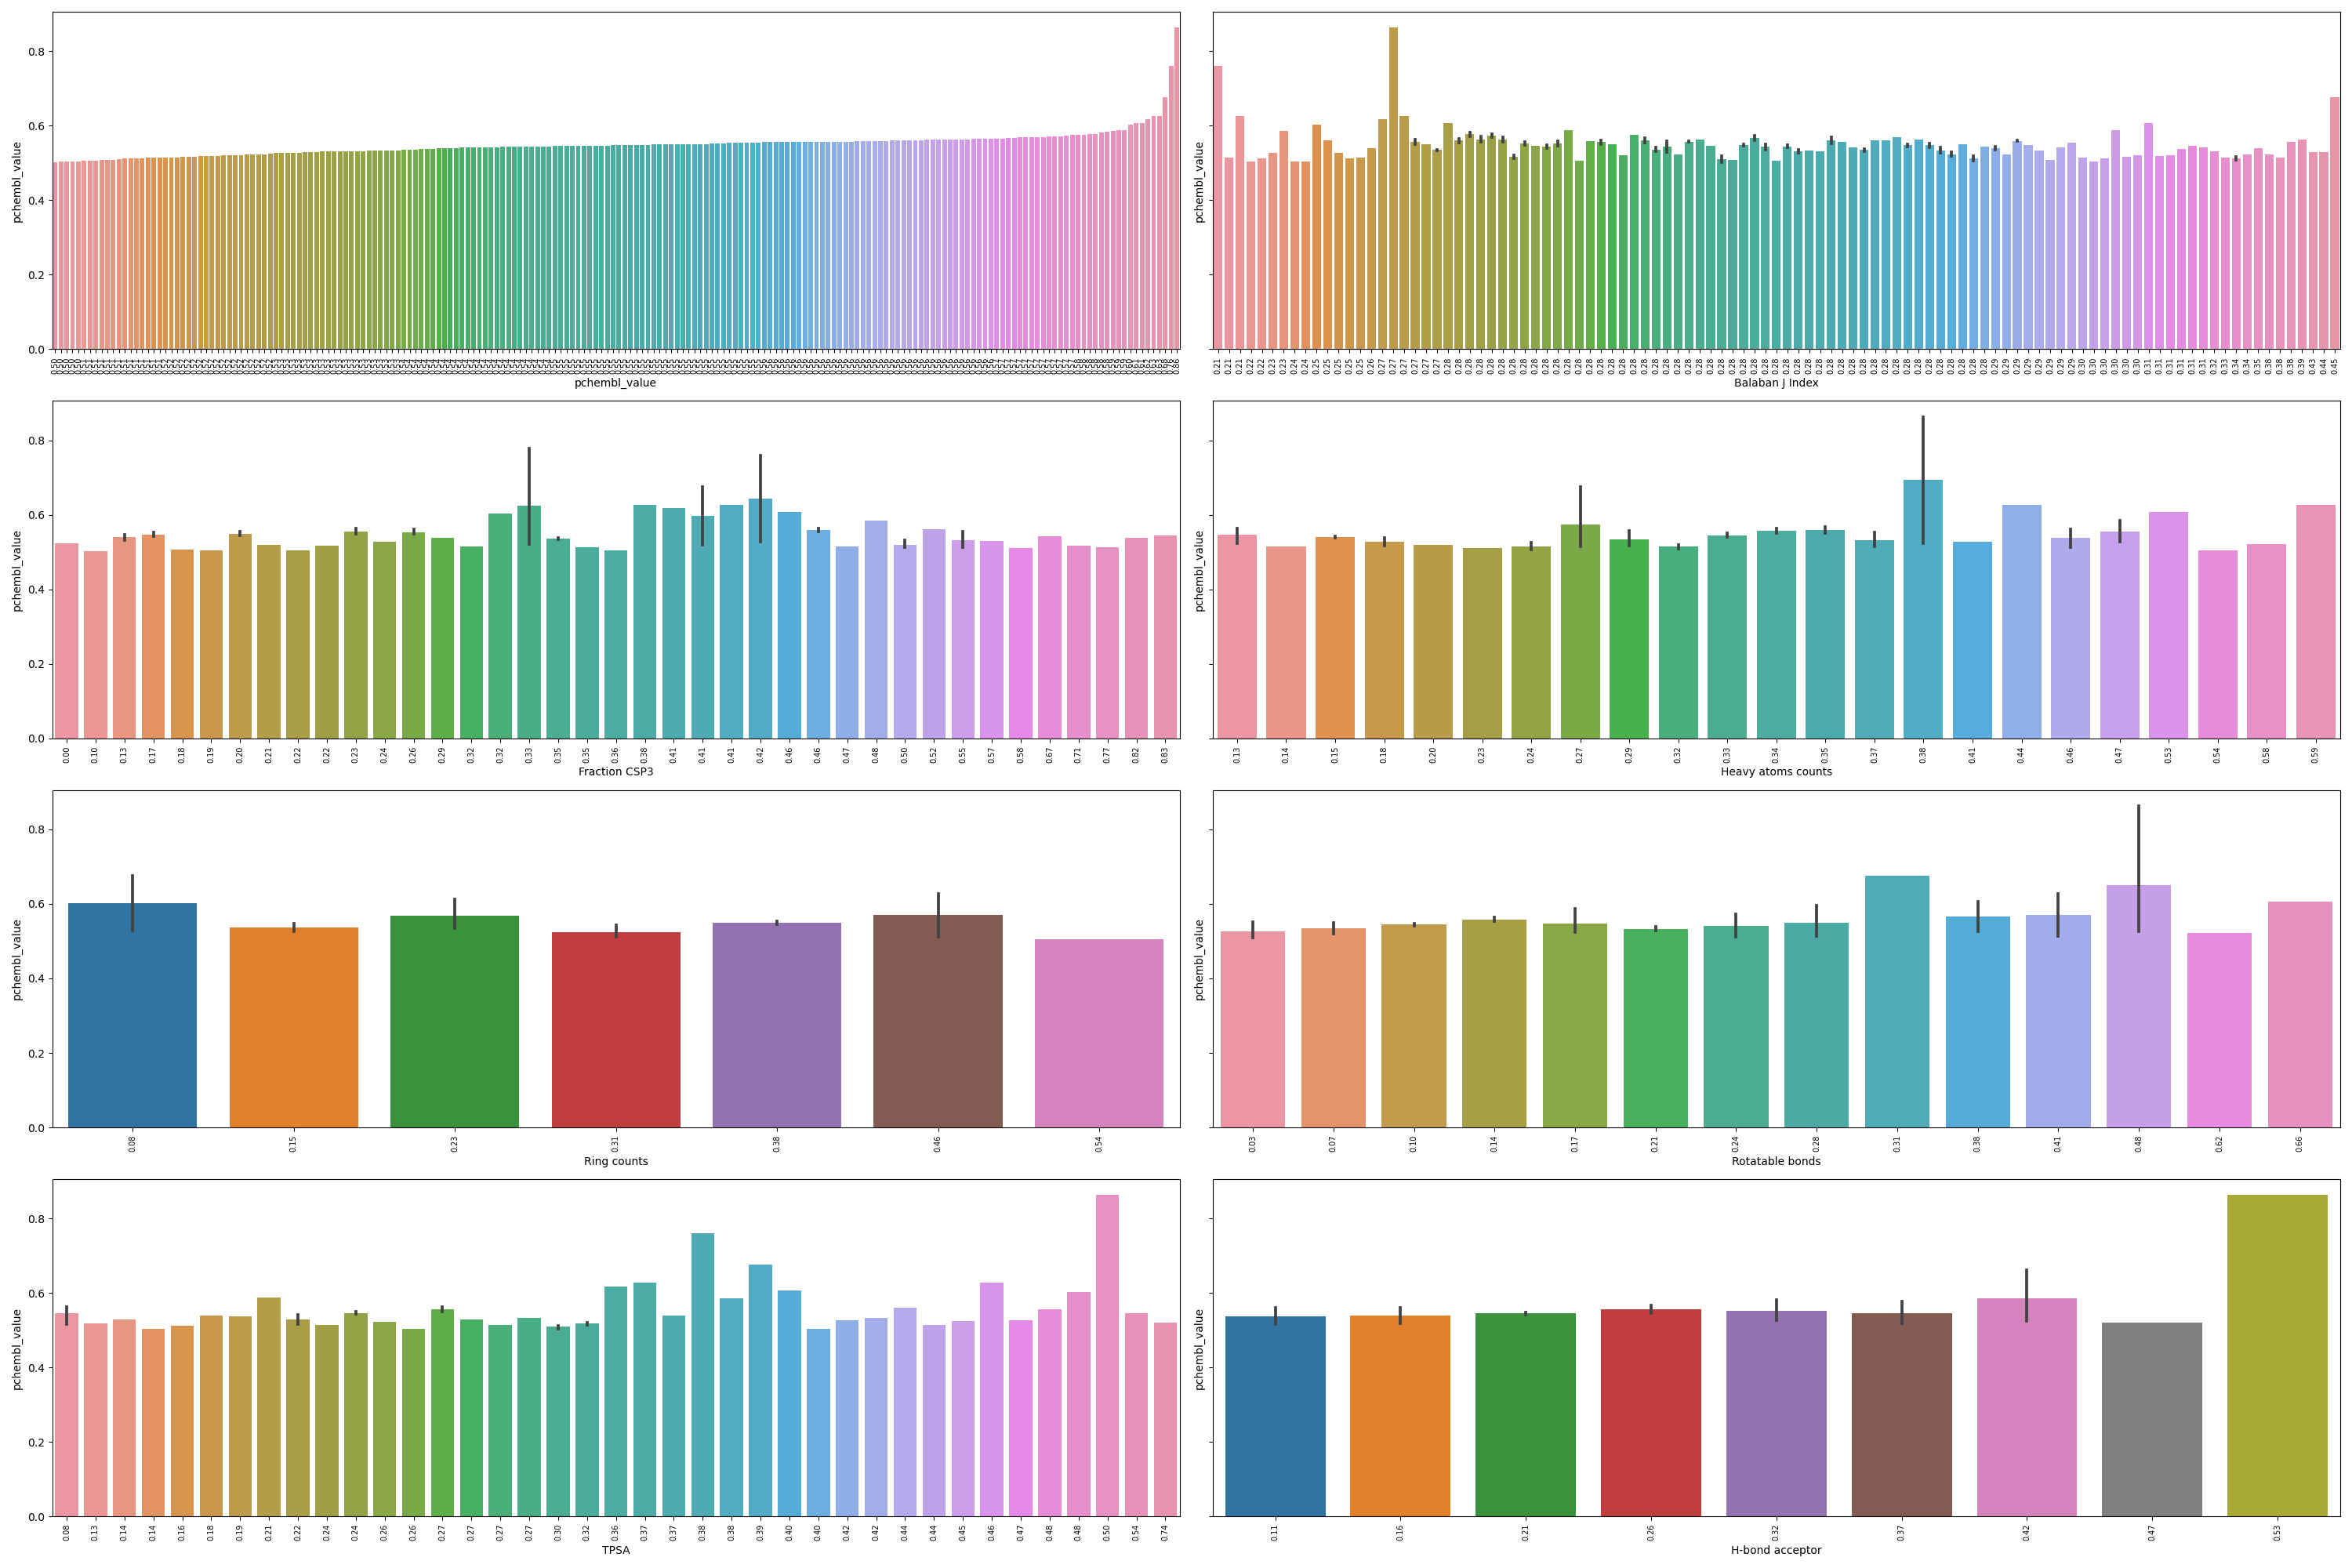
\includegraphics[width=0.9\linewidth, height=4cm]{barplot_matrix_predict_chemdiv.png} 
        \caption{}
        %%\label{fig:subim1}
    \end{subfigure}
    \begin{subfigure}{0.9\textwidth}
        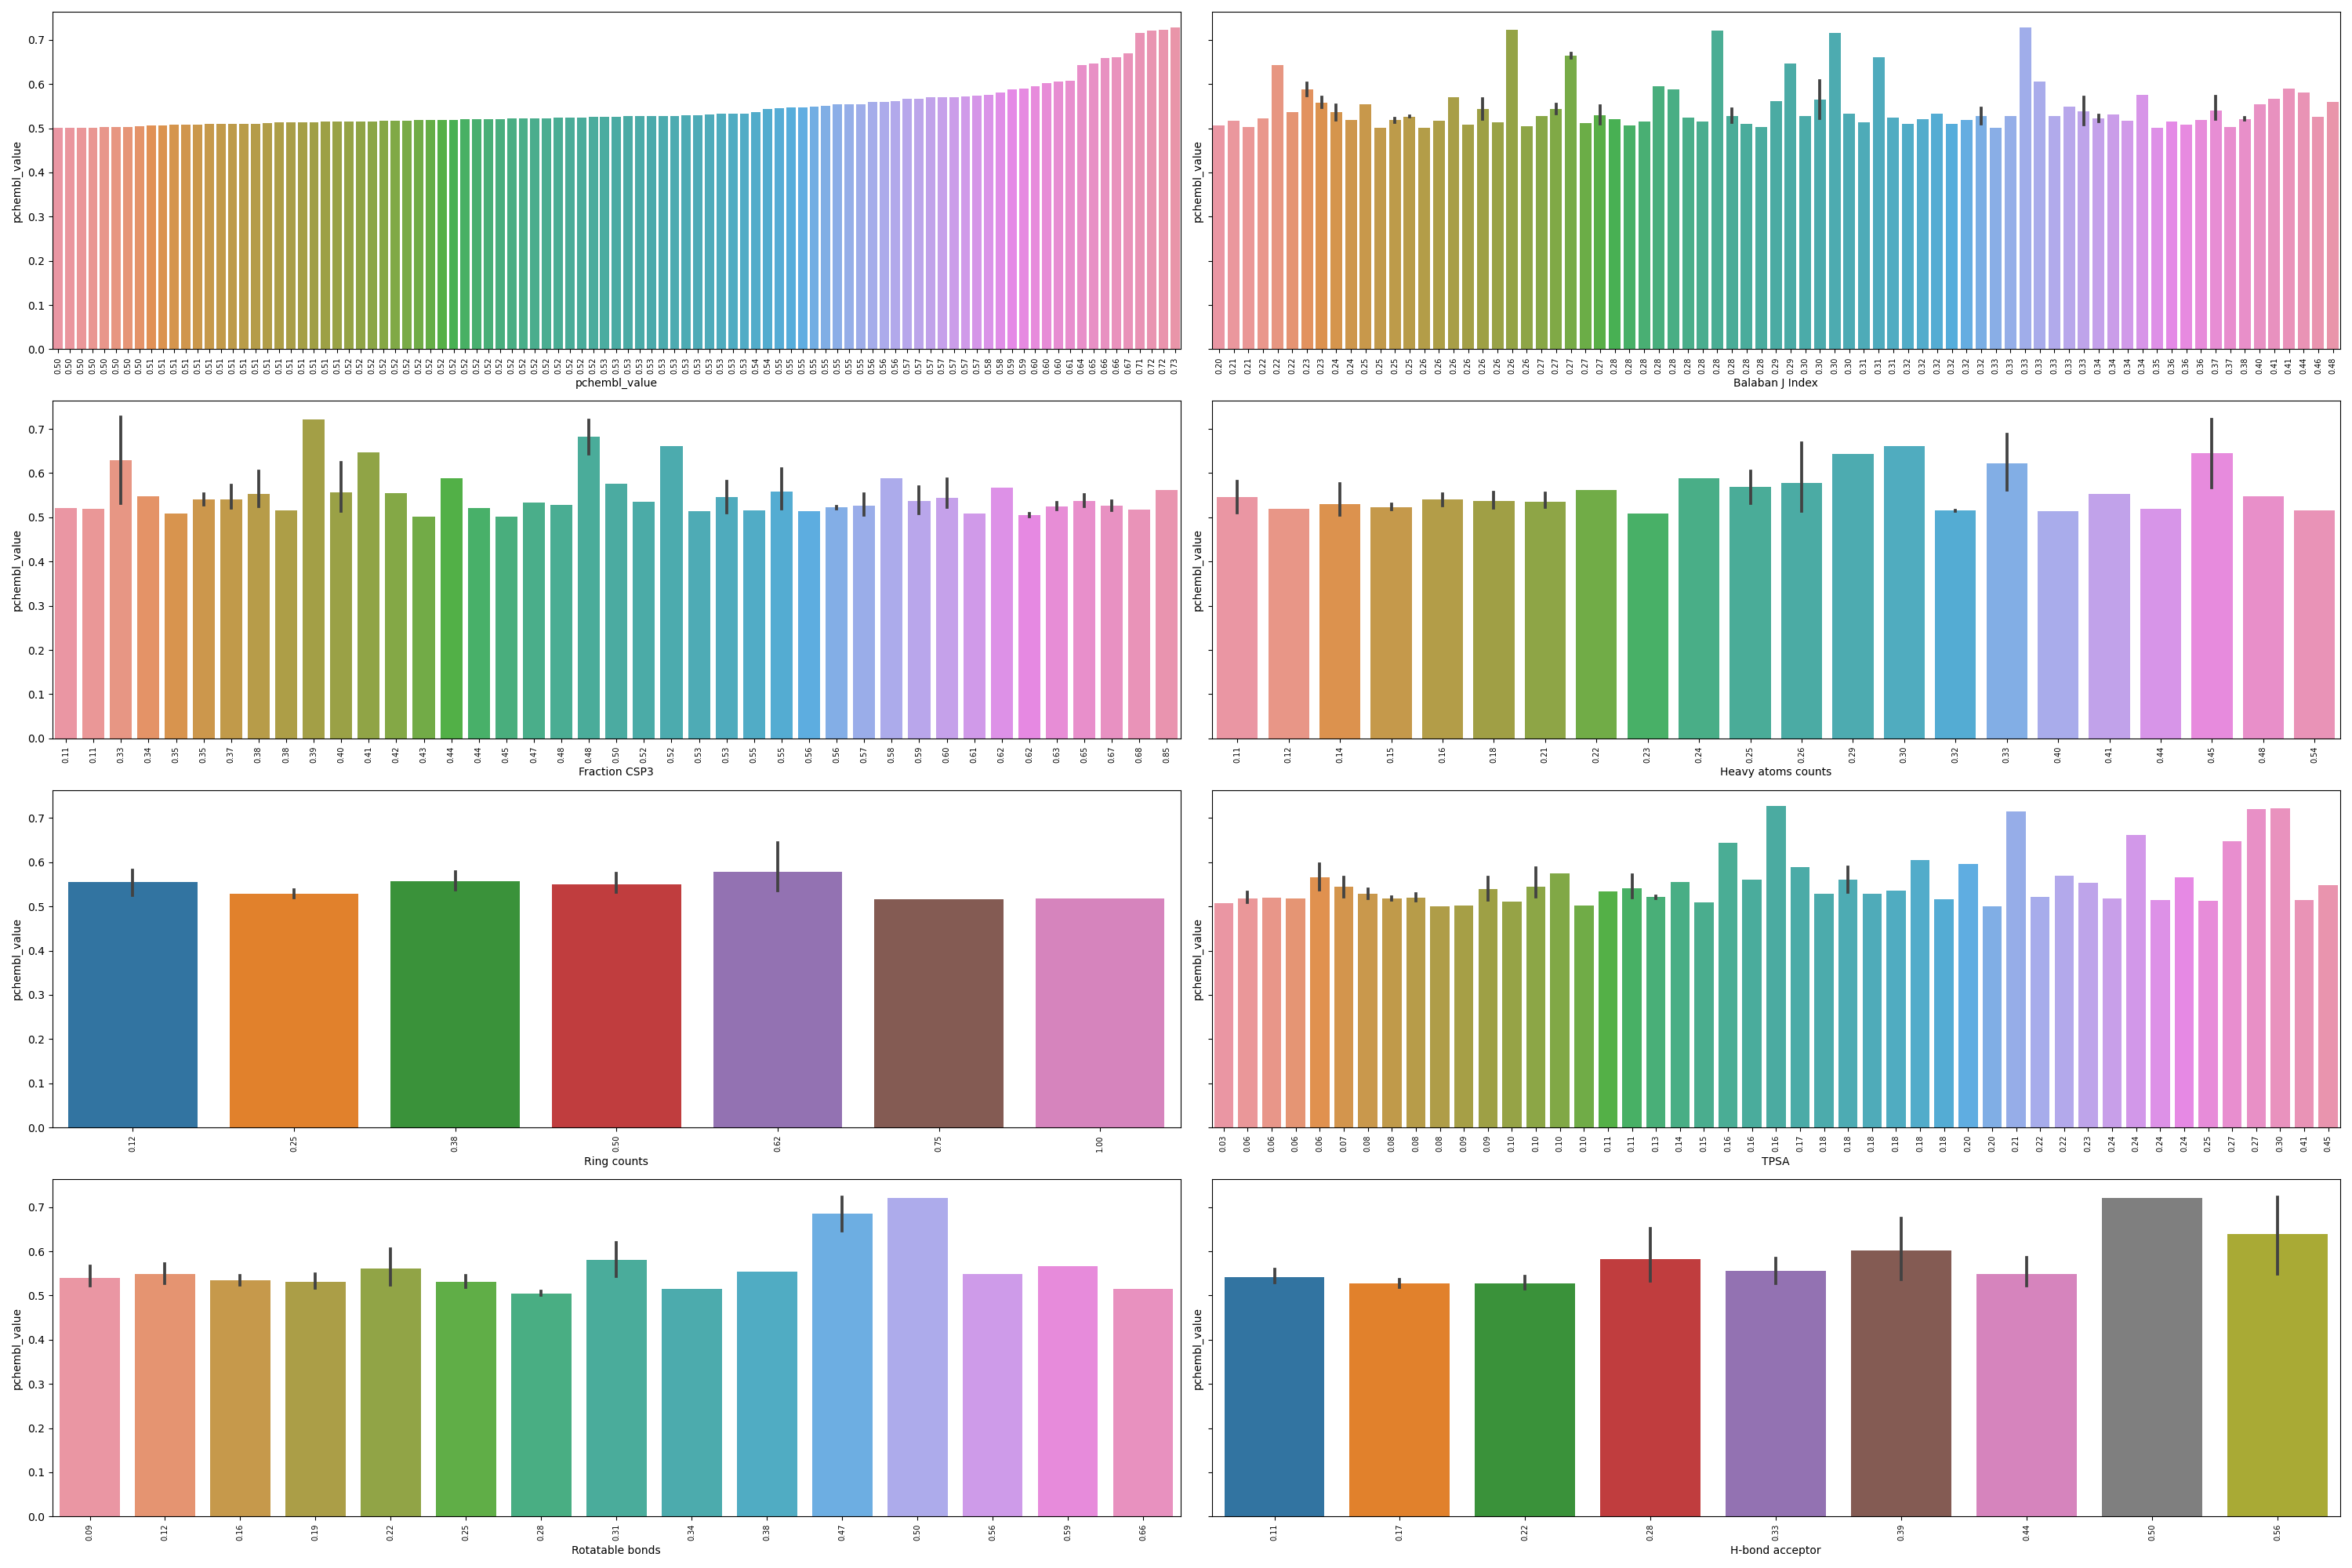
\includegraphics[width=0.9\linewidth, height=4cm]{barplot_matrix_predict_zinc.png}
        \caption{}
        %%\label{fig:subim2}
    \end{subfigure}
    
    \caption{Barplot matrix analysis from predicted results among IC50. (a)Fist predict, Chemdiv (b)Second predict, Zinc }
    \label{Figure17}
\end{figure*}


 We conclude the analysis with a similarity test of the top 10 molecules selected from each of the datasets resulting from the predictions (Table~\ref{Figure14}). Using the Tanimoto coefficient, a score of 1 exactly similarity, while 0 indicates no similarity. It is important to note that in all cases, very low similarity values are observed, with a maximum value of 0.2.

 Upon examining the images of the top 10 molecules from the first set of predictions (Figure{\ref{Figure15}}), the top 10 molecules from the second set of predictions (Figure~\ref{Figure16}), and referring to Table~\ref{Figure14}, we observe that the molecules with the highest similarity values within the results are M1 from Figure~\ref{Figure15} with M5 and M7 from Figure~\ref{Figure16}, both having a value of 0.207. The next best similarity results at value 0.2 , are for M4 on Figure~\ref{Figure15} also with M5 and M7 on Figure~\ref{Figure16}. 
 

\section{Discussion}

When analyzing the results of the different Chemprop trainings, we have used training 4 to make predictions for our study. We considered it to be the most appropriate and well-fitted, as both the MSE, RMSE, and MAE values are the most favorable in this training. Although the highest $R^2$ value was obtained in training 2 with a value of 0.68, the difference between this result and training 4 with an $R^2$ of 0.67 is negligible, so we have decided to proceed with training 4 as the model to predict our results.

The most desviated result from a well-fitted model was observed in training 1, which can be attributed to the fact that this training was performed with a dataframe containing very raw data, with many repeated SMILES, which could have affected the machine learning model. Therefore, we can see how the importance of good data cleaning is reflected in the training results.

Upon analyzing the prediction model versus the trained model, we observe that for the data of greatest interest to us, those with higher IC50 values, the regression line shows an increase in dispersion (see figure). This indicates that our model is not entirely reliable, especially for results where IC50 is crucial for inhibitor discovery.

Regarding the features analyzed in the prediction results based on the correlation of variables, in all three cases analyzed (see Figures~\ref{Figure8},~\ref{Figure10},~\ref{Figure13}), we can see a strong correlation between the MW and Heavy Atom Count features. This may be due to the fact that heavier molecules tend to have more heavy atoms.

As for the relationship between variables and the IC50 value, the analysis suggests that in none of the three datasets is there a strong correlation with this variable, particularly in the training dataset. This indicates that a strong interaction activity is not significantly correlated with these chemical characteristics. Nonetheless, in Figure~\ref{Figure17} of the predictions, we can observe how it supports the results of the correlation heatmap, where it is evident that the variables H-bond acceptor, TPSA, Heavy Atom Counts, and Rotatable Bonds are the ones with the highest values.

Finally, regarding the similarity analysis, we have been unable to obtain conclusive results because the maximum similarity values are very low and, therefore, unreliable. However, we have observed that molecules M5 and M7 from the second training set, based on zinc data, are highly similar. We have confirmed this initially through Figure X and secondly by noticing that they share the same similarity values with a specific molecule from the first Chemdiv training set. This could serve as a starting point for further research to understand the characteristics of these molecules.

We have also noticed some similarity among all molecules in the Chemdiv database, as they interact with very little difference in similarity compared to molecules in the zinc database. This is attributed to the fact that all these molecules originate from a cisteine protease warheads database, hence sharing similar features.

\FloatBarrier
\section{Conclusions}

After conducting an analysis and training algorithms of ANN that allowed us to identify patterns and improve the stability of the prediction model. However, even though we have made progress in this regard, the results have not yet reached the necessary optimization to ensure full data reliability. This suggests the importance of conducting deeper and more comprehensive training to achieve a more precise adaptation of the model and enhance its predictive capacity.

Regarding the search for patterns through the correlation between molecular features, our results indicate that we have not found a strong enough correlation between the analyzed variables and inhibitory activity. This finding leads us to consider the need to expand our research, exploring a broader set of molecular features to delve deeper into the relationship between these features and inhibitory activity, which could shed light on new markers and predictors.

Finally, despite the overall unfruitful search for similarities, we highlight the interesting discovery of two highly similar molecules in the zinc database, both with elevated IC50 values. This discovery could serve as a starting point for further investigations exploring the relationship between these molecules and their ability to inhibit cysteine proteases, thus opening new avenues of study in this field.

In summary, this study highlights the potential of machine learning, particularly artificial neural networks (ANNs), as a powerful tool for streamlining the drug discovery process by facilitating the identification of promising compounds for covalent inhibition. Although the results may not have yielded effective inhibitors in this specific context, this research underscores the value of ML technology in exploring new avenues and approaches in the quest for innovative therapies.

\appendix

\section{Acknowledgments}

I would like to express my gratitude to my project supervisor, Jordi Villa, for guiding me throughout the project, and to my partner and family for their unwavering support during the entire process.

\section{Data availability}

The code used for this study is available on the following GitHub repository: \href{https://github.com/carlafeliu/TFM}{https://github.com/carlafeliu/TFM}

%%\section{Abbreviations}

\section{References}
\bibliographystyle{unsrt} 
\bibliography{library_tfm}


\end{document}

%%\endinput

